\documentclass[hideothersubsections]{beamer}
\usepackage{pgfpages}
\usepackage[absolute,overlay]{textpos}
\usepackage[makeroom]{cancel}
\setbeameroption{show notes on second screen=right}


\newcommand\parallelcontent[2]{
	\begin{columns}[t]
		\column{0.48\textwidth} #1
		\column{0.48\textwidth} #2
	\end{columns}
}
\newcommand\parallelitem[2]{
	\parallelcontent
	{\begin{itemize} \item #1 \end{itemize}}
	{\begin{itemize} \item #2 \end{itemize}}
}

\mode<presentation> {

% The Beamer class comes with a number of default slide themes
% which change the colors and layouts of slides. Below this is a list
% of all the themes, uncomment each in turn to see what they look like.

%\usetheme{default}
%\usetheme{AnnArbor}
%\usetheme{Antibes}
%\usetheme{Bergen}
%\usetheme{Berkeley}
%\usetheme{Berlin}
%\usetheme{Boadilla}
%\usetheme{CambridgeUS}
%\usetheme{Copenhagen}
%\usetheme{Darmstadt}
%\usetheme{Dresden}
%\usetheme{Frankfurt}
%\usetheme{Goettingen}
%\usetheme{Hannover}
%\usetheme{Ilmenau}
%\usetheme{JuanLesPins}
%\usetheme{Luebeck}
%\usetheme{Madrid}
%\usetheme{Malmoe}
%\usetheme{Marburg}
%\usetheme{Montpellier}
\usetheme{PaloAlto}
%\usetheme{Pittsburgh}
%\usetheme{Rochester}
%\usetheme{Singapore}
%\usetheme{Szeged}
%\usetheme{Warsaw}

% As well as themes, the Beamer class has a number of color themes
% for any slide theme. Uncomment each of these in turn to see how it
% changes the colors of your current slide theme.

%\usecolortheme{albatross}
%\usecolortheme{beaver}
%\usecolortheme{beetle}
%\usecolortheme{crane}
%\usecolortheme{dolphin}
%\usecolortheme{dove}
%\usecolortheme{fly}
%\usecolortheme{lily}
%\usecolortheme{orchid}
%\usecolortheme{rose}
%\usecolortheme{seagull}
\usecolortheme{seahorse}
%\usecolortheme{whale}
%\usecolortheme{wolverine}

%\setbeamertemplate{footline} % To remove the footer line in all slides uncomment this line
%\setbeamertemplate{footline}[page number] % To replace the footer line in all slides with a simple slide count uncomment this line

\setbeamertemplate{navigation symbols}{\hskip6pt\raisebox{2pt}{\color{black}\insertframenumber/ \inserttotalframenumber}}

%\setbeamertemplate{navigation symbols}{} % To remove the navigation symbols from the bottom of all slides uncomment this line
}
\usefonttheme[onlysmall]{structurebold}
\usepackage{textpos}
\usepackage{graphicx} % Allows including images
\usepackage{booktabs} % Allows the use of \toprule, \midrule and \bottomrule in tables

%----------------------------------------------------------------------------------------
%	TITLE PAGE
%----------------------------------------------------------------------------------------

\title[]{Theoretical and Numerical Studies of Efimov States} % The short title appears at the bottom of every slide, the full title is only on the title page

\author{Kajsa-My Blomdahl} % Your name
\institute[SU] % Your institution as it will appear on the bottom of every slide, may be shorthand to save space
{
Stockholms Universitet \\ % Your institution for the title page
\medskip
\textit{kajsamy.blomdahl@fysik.su.se} % Your email address
}
\date{\today} % Date, can be changed to a custom date
%\logo{
\includegraphics[height=1.0cm]{logga}}

\begin{document}
	
\begin{frame}
	\titlepage
	\note[item]{Hi, my name is Kajsa-My Blomdahl, I study Efimov Physics, which is encapsulte a number of effects that appear in the quantum 3BP.}
\end{frame}

%\section[Outline]{Outline}
\frame{\tableofcontents[hideallsubsections]
\note[item]{To understand important features of the quantum 3BP I will start by introduce a few concepts from quantum scattering of 2 particles.}}

%----------------------------------------------------------------------------------------
%	PRESENTATION SLIDES
%----------------------------------------------------------------------------------------

\section{Introduction}
\subsection{Two-body Interactions}
\begin{frame}
\frametitle{Two-body (2-b) Interactions}
\begin{itemize}
	\item<1-> Atomic collisions in the ultra cold regime
	\item<2-> Quantized orbital angular momenta $l=0,1,2$, are referred to as \alert<3>{$s$-waves}, $p$-waves and $d$-waves etc.
	\item<4-> 2-b scattering in this regime is governed by a parameter called the \alert{s-wave scattering length $a$}
\end{itemize}
\note[item]<1>{Atomic interactions are, essentially, pair-wise and short-ranged, which means that they interact when they are close to each other.}
\note[item]<2>{At very low energies, atoms behave like point particles and have quantized orbital angular momenta l. The quantum numbers l = 0,1,2, associated with an atom, are referred to as s-waves, p-waves and d-waves, and so on}
\note[item]<3>{In the ultracold regime s-wave collisions dominate (because higher partial waves are reflected by the centrifugal barrier in the SE)}
\note[item]<4>{Two-body scattering in this regime is solely governed by a single parameter called the s-wave scattering length a, or just scattering length for short}
\end{frame}

%-------------------------------------------

\subsection{Scattering Length}
\begin{frame}
\frametitle{Scattering Length}
\invisible<5>{
\begin{itemize}
	\item<1-4,6->Definition:
	\begin{equation*}
	a = \lim_{k \to 0} -\frac{\tan\alert<2>{\delta_0(k)}}{k}
	\end{equation*}
	\item<3-4,6-> Characterizes the strength of the interparticle interaction
	\item<4,6-> The sign of $a$ and the effective interaction
	\item<6-> \alert<6>{Negative} $a$ $\rightarrow$ \alert<6>{attractive} effective interactions
	\item<7-> \alert<7>{Positive} $a$ $\rightarrow$ \alert<7>{repulsive} effective interactions
	\item<8-> For \alert<8>{$|a| \rightarrow \infty$} the interaction is called \alert<8>{resonant} 
\end{itemize}}
\only<5>{
	\vspace*{-4.5cm}
	\centering
	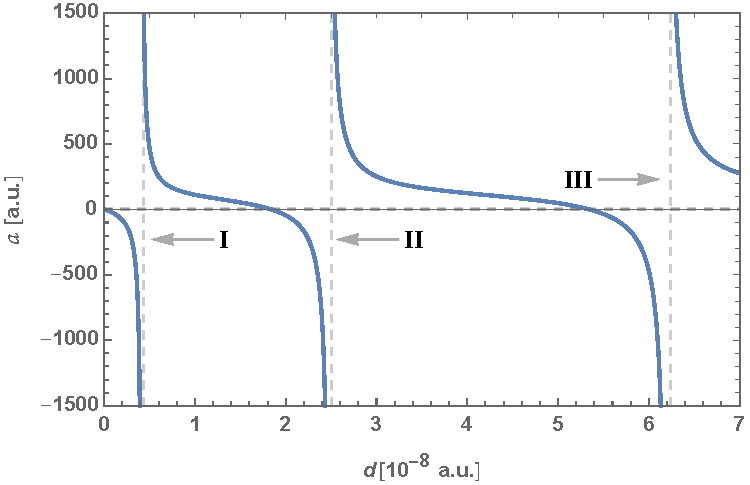
\includegraphics[width=1.0\linewidth]{scattering_new.pdf}}

\note[item]<1>{The s-wave scattering length is defined in the low-energy limit as}
\note[item]<2>{where $\delta$ is the s-wave phase shift of the outgoing wave (and $k$ is the wave number $=\sqrt{2\mu E}/\hbar$)}
\note[item]<3>{The scattering length characterizes the strength of the interaction In the absence of an interaction, the phase shift is simply zero and the outgoing scattered wave is in phase with the incoming wave. Any interaction will cause a dephasing between the outgoing and incoming waves. The strongest dephasing occur when is $\pi/2$ $a$ will then diverge.}
\note[item]<4>{The sign of $a$ carries information about wether the effective interaction is attractive or repulsive. If the two-body interaction has no bound states $a$ is negative. However if the interaction has one or more bound state $a$ can be both positve and negative.}
\note[item]<5>{To illustrate this I have finetuned a model two body potential by changing the depth of the potential. Here we have $a$ on the y-axis and the depth $d$ of the attractive 2b-potential on the x-axis.}
\note[item]<6>{Negative scattering lengths correspond to attractive effective interactions, meaning the scattered wave is being pulled in by the potential}
\note[item]<7>{Positive scattering lengths correspond to repulsive effective interactions, meaning the scattered wave is being pushed out by the potential}
\note[item]<8>{When the magnitude of $a$ $\rightarrow \infty$ we say that the interaction is resonant. In this case the interaction is fully characterized by the scattering length, which is much larger than the interaction range of the particles.}
\end{frame}

%-------------------------------------------

\subsection{Universality}
\begin{frame}
\frametitle{Universality in 2-b systems}
\only<1->{
\begin{block}{2-b scattering}
	Particles with large $|a|$ in the low-energy regime have universal properties
\end{block}}

\only<2->{
\begin{block}{Universal properties ... In what sense?}
	Depend on the scattering length alone and not on the details of the short-range interaction
\end{block}}

\only<3->{
\hypertarget{dimer}
{\hyperlink{lastres}{\beamergotobutton{Results}}}
\begin{block}{Example: 2-b binding energy for 2 identical bosons}
	\begin{equation*}
	E_D = \frac{\hbar^2}{m a^2}
	\end{equation*}
\end{block}}
\note[item]<1>{Particles with large scattering lengths in the low-energy regime are interesting because they have universal properties. }
\note[item]<2>{What do we mean by universal? It means that they depend on the scattering alone and not on the details of the short-range interction, which means all bosons behave in the same way it does not matter what atomic species we look at}
\note[item]<3>{For example: }
\end{frame}

%-------------------------------------------

\subsection{The Efimov Effect}
\begin{frame}
\frametitle{Efimov's Prediction}
\begin{columns}
	\column{0.4\textwidth}
	\begin{itemize}
	\only<1>{\item Resonant 2-b forces give rise to bound energy levels in 3-particle systems}
	\only<2>{\item When $|a| \rightarrow \infty$ a universal long-range 3-body attraction emerge}
	\only<3->{\item<3-> Scale transformation constant $$\lambda=e^{\pi/\alert<4>{s_0}} \approx 22.7$$
	\item<4-> \alert<4>{$s_0 \approx 1.00624$} 
	\item<5-> Size scaling: $$\rho^{n+1}/\rho^{n} \approx \lambda$$
	\item<6-> Energy scaling: $$E_T^{n+1}/E_T^{n} \approx \lambda^2 \approx 515$$}
\end{itemize}
\column{0.6\textwidth}
\only<1,3->{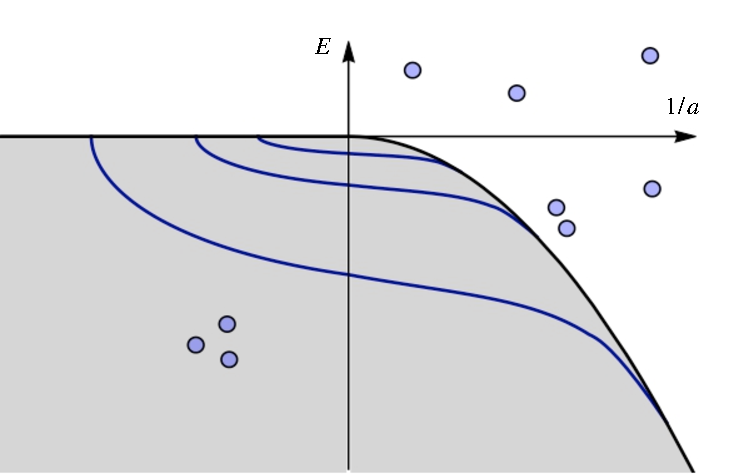
\includegraphics[width=1.0\linewidth]{efimov1}}
\only<2>{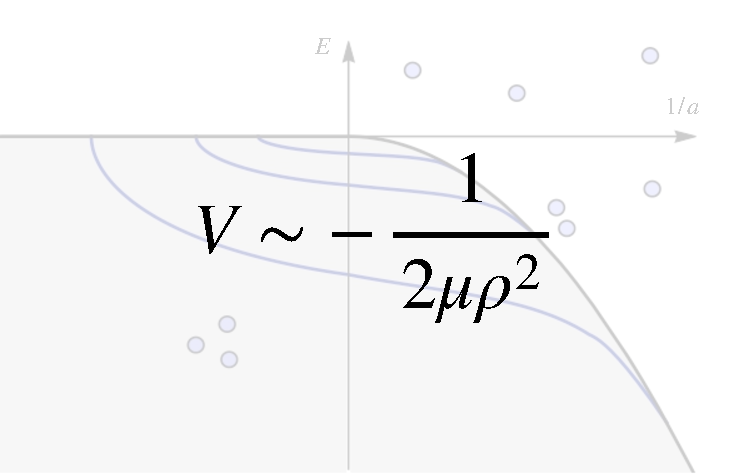
\includegraphics[width=1.0\linewidth]{efimov2}}
\end{columns}
\note[item]<1>{In the 1970 Vitaly Efimov predicted that resonant can give rise to a series of bound energy levels in 3-particle systems, which we now call Efimov states}
\note[item]<2>{When the short-ranged two-body forces approached resonance, he found a universal long-range three-body attraction emerging, giving rise to an infinite number of trimer states with binding energies obeying a discrete scaling law at resonance.}
\note[item]<3>{The Efimov states have universal properties. For three identical bosons are that the size and energy of successive trimer states in the resonant limit are related by a scale transformation with a constant $\lambda=e^{\pi/s_0} \approx 22.7$}
\note[item]<4>{Is a universal constant in Efimov physics, which I will return to later}
\note[item]<5>{The ratio of the size of two succesive Efimov states is given by the constant lambda}
\note[item]<6>{while the ratio of the energy of two succesive Efimov states scale geometrically with lambda}
\end{frame}

%-----------------------------------------------

\begin{frame}
\frametitle{The Peculiar Efimov Effect}
\only<1>{} 
\begin{itemize}
\item<2-> The size of each Efimov state (ES) $\gg$ the interaction range ($r_0$) between the individual particle pairs $\rightarrow$ QM effect
\item<3-> When $a \rightarrow \pm\infty$ the $\#$ of ES $ \rightarrow \infty$
\item<4-> The $\#$ of ES is \alert<4>{reduced} as the 2-b interaction is made more attractive
\item<5-> The effect is universal and can \textit{in principle} be observed in any QM system 
\end{itemize}
\note[item]<1>{The Efimov effect is remarkable in many ways}
\note[item]<2>{Because the size of each Efimov state is much larger than the force-range between the individual pairs it means we are dealing with a pure quantum mechanical effect}
\note[item]<3>{When the magnitude of scattering length approach infty, there is an infinite number of Efimov states}
\note[item]<4>{$\#$ of 3-b bound states is \textit{reduced} as the 2-b interaction is made more attractive.}
\note[item]<5>{The effect is universal, which means that the states emerge irrespective of the nature of the 2-b forces and can in principle be observed in all quantum mechanical systems}
\end{frame}

%------------------------------------------------

\section{Theoretical Approach}
\begin{frame}
\frametitle{Theoretical Approach}
\begin{description}
\item<2->[Q:] 3-Particles, What Is The Problem?
\item<3->[A:] The configuration space (CS) for the 3BP is 9D and highly non-trivial ...
\item<4->[Solution:] Reduce the number of dimensions!
\end{description}
\note[item]<1>{The 3BP is famous for being hard to solve}
\note[item]<2>{So why is the problem of 3 so complex?}
\note[item]<3>{Well, the configuration space for the 3BP is 9D and highly non-trivial ...}
\note[item]<4>{So what we want to do is to reduce the dimensionality of the problem}
\end{frame}

%---------------------------------------------------------
\subsection{Step 1}
\begin{frame}
\frametitle{Step 1: Relative Coordinates}
\begin{itemize}
	\item<1->{Separate out CoM by introducing relative coordinates}
	\item<3->{Choice: Mass-normalized \alert<4>{Jacobi coordinates}}
	\item<2->{CS $\rightarrow$ 6D}
\end{itemize}
\vspace*{1cm}
\only<4>{
	\centering
	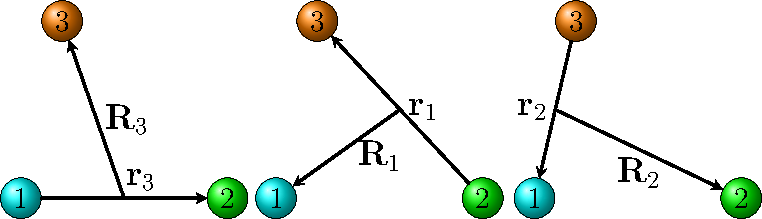
\includegraphics[width=0.9\linewidth]{jacobi_p.pdf}}
\note[item]<1>{The first step to reduce the number of D is to separate out the CoM by introducing relative coordinates.}
\note[item]<2>{CoM motion decouples from the internal motion in the SE the configuration space is effectively reduced to 6D}
\note[item]<3>{For internal coordinates we choose a Mass-Normalized Jacobi coordinates}
\note[item]<4>{$\mathbf{r}$ is the vector that connects two of the particles and $\mathbf{R}$ connects the CoM of these two particles with the third particle}
\note[item]<4>{Particle permutations are easily performed using these coord.}
\end{frame}

%---------------------------------------------------------

\subsection{Step 2}
\begin{frame}
\frametitle{Step 2: Hyperspherical Coordinates}
\begin{itemize}
	\item<2->{Combine $\mathbf{r}_k$ and $\mathbf{R}_k$ into a 6D position vector in $\mathbb{R}^6$}
	\item<3->{Hyperspherical coordinates: $\rho$ and $\Omega$ $$\rho = (\mathbf{r}^2+\mathbf{R}^2)^{1/2}$$}
	\item<4-> Separate internal and external coordinates
	\item<5-> For $J=0$ only \alert{internal coordinates} matter $\rightarrow$ 3D Schr{\"o}dinger equation (SE)
\end{itemize}
\note[item]<1>{Step 2 in simplifying the problem of three particles is to introduce hyperspherical coordinates}
\note[item]<2>{The general idea is to combine the components of the two Jacobi vectors into a single six-dimensional position vector q, which represents a point in R6.}
\note[item]<3>{The hyperspherical coord. of this point are given by the hyperradius ρ and five hyperangles $\Omega$.}
\note[item]<3>{The hyperradial coordinate is both rotationally and permutationally invariant and is defined as the square root of the sum of the squared Jacobi vectors.}
\note[item]<3>{The hyperangles can be defined in many ways and  I will not go in to the details here.}
\note[item]<4>{At any instant, three particles form a plane in R3. We can define the internal motion of the particles within this plane in terms of the hyperradial coordinate (size) and two of the angles(shape and particle permutation). The three other angles relate rotations of this plane in a space fixed system.}
\note[item]<4>{The three other angles relate rotations of this plane in a space fixed system.}
\note[item]<5>{When the orbital angular momenta J=0 only the internal coordinates matter and we are left with a 3D SE for the internal motion}
\end{frame}

%---------------------------------------------------------

\subsection{Step 3}
\begin{frame}
\frametitle{Step 3: The Adiabatic Representation}
\begin{itemize}
\item<2->{
\hypertarget{SE}
The hyperspherical SE:
\begin{equation*}
\bigg(-\frac{1}{2 \mu}\frac{\partial^2}{\partial \rho^2} +\alert<5>{ \frac{ \alert<3>{\Lambda}^2 + \frac{15}{4}}{2 \mu \rho^{2}}+ V}\bigg)\psi = E\psi
\end{equation*}}

\item<4-> Trick: Treat $\rho$ as an adiabatic parameter! 

\item<5->{
\hypertarget<5>{supplemental}
Solve the adiabatic eq.
\begin{equation*}
\alert<5>{H_{ad}}\Phi_{\nu}{(\rho;\Omega)} = \alert<6>{U_{\nu}{(\rho)}}\Phi_{\nu}(\rho;\Omega)
\end{equation*}}
\item<6->$\rightarrow$ \alert<6>{3-body BO-like potential}
\end{itemize}
\hyperlink{matrix}{\beamerbutton{Numerical Approach}}
\hyperlink{sum}{\beamerbutton{Exact rep.}}
\note[item]<1>{Now we move on to the final step (in the simplification of the 3BP)}
\note[item]<2>{After a clever rescaling of the wfn, the hyperspherical SE can be written like this}
\note[item]<3>{Where lambda is the generalized angular momenta}
\note[item]<4>{Now, the trick is to treat the hyperradius as an adiabatic parameter!}
\note[item]<4>{That is, we fix $\rho$ in a Born-Oppenheimer like manner}
\note[item]<5>{And solve the remaining adiabatic eigenvalue equation}
\note[item]<6>{In this way we obtain the three-body equivalent of a BO potential.}
\end{frame}

%------------------------------------
\begin{frame}
\frametitle{Step 3: The Adiabatic Representation cont.}
\begin{itemize}
	\item<1->{The total wave function is represented in terms of \alert<2>{adiabatic states}
	\begin{equation*}
	\psi_{n}(\rho,\Omega) = \alert<3>{\sum_{\nu=0}^{\infty} F_{n\nu}(\rho)\alert<2>{\Phi_{\nu}(\rho;\Omega)}}
	\end{equation*}}
	\item<4->{
	\hypertarget{sum}	
	The hyperradial eigenvalue equation 
	\scriptsize
	\begin{equation*}
		\bigg(-\frac{1}{2 \mu}\frac{\partial^2}{ \partial \rho^2} + \alert<5->{U_{\mu} - \frac{1}{2\mu}Q_{\mu\mu}} \bigg)F_{n\mu} -\frac{1}{2\mu}\bigg(\sum_{\nu\neq\mu}2P_{\mu\nu}\frac{\partial}{\partial\rho} + Q_{\mu\nu} \bigg)F_{n\nu}= E_nF_{n\mu}
	\end{equation*}}
\end{itemize}
\only<6>{
\begin{textblock*}{80mm}(32mm,0.35\textheight)
	\begin{exampleblock}{Three-body effective potentials}
		\begin{equation*}
		W_{\nu}(\rho) = U_{\nu}(\rho)-\frac{1}{2\mu}Q_{\nu \nu}(\rho) = U_{\nu}(\rho)-\frac{1}{2\mu}P_{\nu \nu}^2(\rho)
		\end{equation*}
	\end{exampleblock}
\end{textblock*}}
\only<7->{
	\begin{textblock*}{80mm}(32mm,0.35\textheight)
		\begin{exampleblock}{Three-body effective potentials}
			\begin{equation*}
			W_{\nu}(\rho) = U_{\nu}(\rho)-\frac{1}{2\mu}Q_{\nu \nu}(\rho) \approx U_{\nu}(\rho)-\xcancel{\frac{1}{2\mu}P_{\nu \nu}^2(\rho)}
			\end{equation*}
		\end{exampleblock}
\end{textblock*}}
\hyperlink{SE}{\beamerbutton{SE}}
\note[item]<1>{Now, in this way the total wfn can be represented by a sum of adiabatic states}
\note[item]<2>{(shown in red)}
\note[item]<3>{If we substitute this sum into the 3-b SE (klick on link)}
\note[item]<4>{We will get an exact representation of the 3-body SE if all couplings are included}
\note[item]<5>{The focus of my work has been on this part of this eq.}
\note[item]<6>{In the adiabatic approximation we define the three-body effective potentials are defined as}
\note[item]<6>{These potentials are used for determining the single channel solutions of (below)}
\note[item]<7>{In this talk I will not explain how the second term is calculated, in the calculations I have performed it is small and we will ignore it from here on}
\end{frame}

%------------------------------------------------------
\section{Effective Potentials}
\subsection{The Asymptotic Limit}
\begin{frame}
\frametitle{Convergence In the Asymptotic Limit}
\begin{columns}
\column{0.46\textwidth}
\vskip-45pt
\visible<2-5>{\begin{block}{For $a<0$:}
		\begin{equation*}
		W_{\nu}(\rho) \xrightarrow{ \rho \to \infty}\frac{\lambda(\lambda+4)+\frac{15}{4}}{2\mu \rho^2}
		\end{equation*}
\end{block}
\vspace{1.35cm}}
\visible<4-5>{\begin{block}{For $a>0$:}
		\begin{equation*}
		W_{\nu}(\rho) \xrightarrow{ \rho \to \infty} E_{2b} +\frac{l(l+1)}{2\mu \rho^2}
		\end{equation*}
	\end{block}
	\hyperlink<5->{finite}{\beamerbutton{Jump to Results}
	\hypertarget<5->{asymptotic}}}
\column{0.54\textwidth}
\raggedright
\visible<3-5>{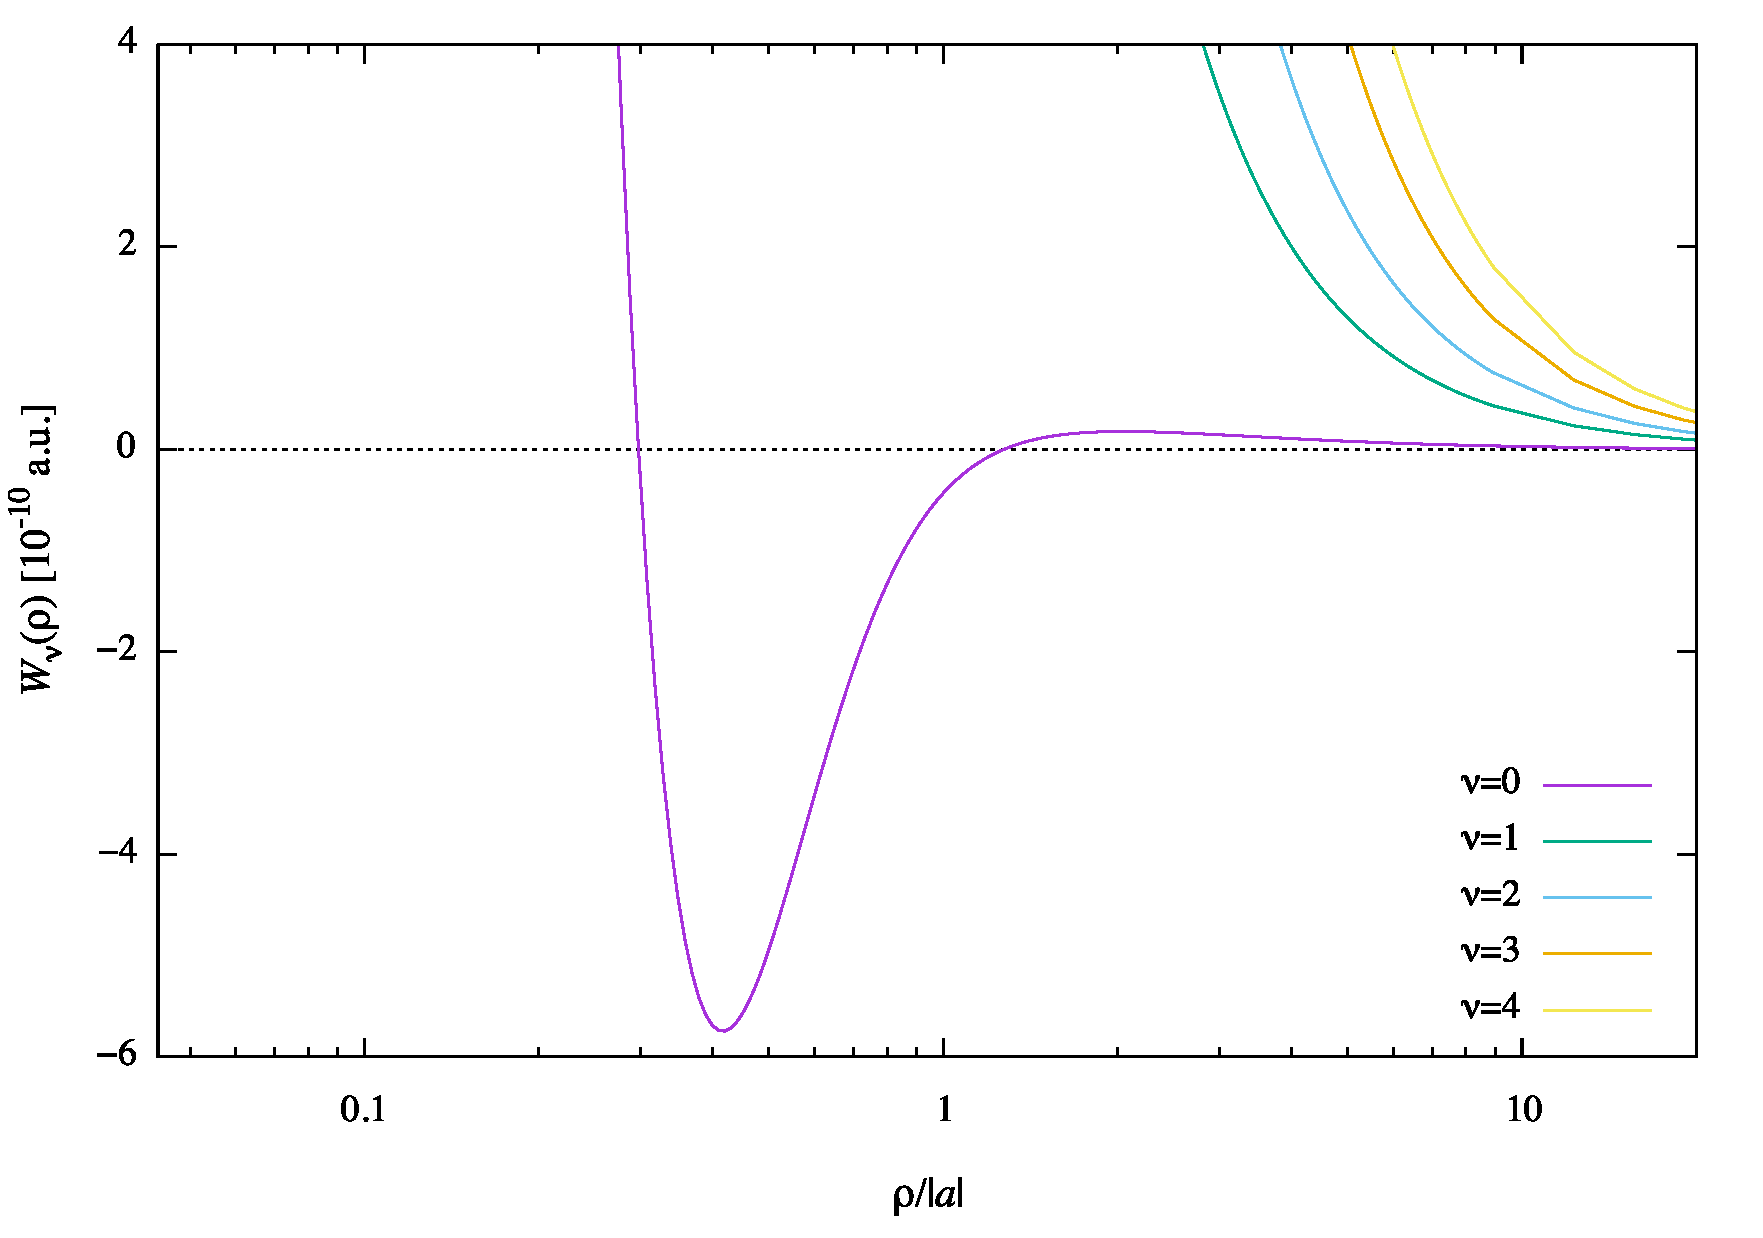
\includegraphics[width=1.0\linewidth]{Wneg.pdf}\\}
\visible<5>{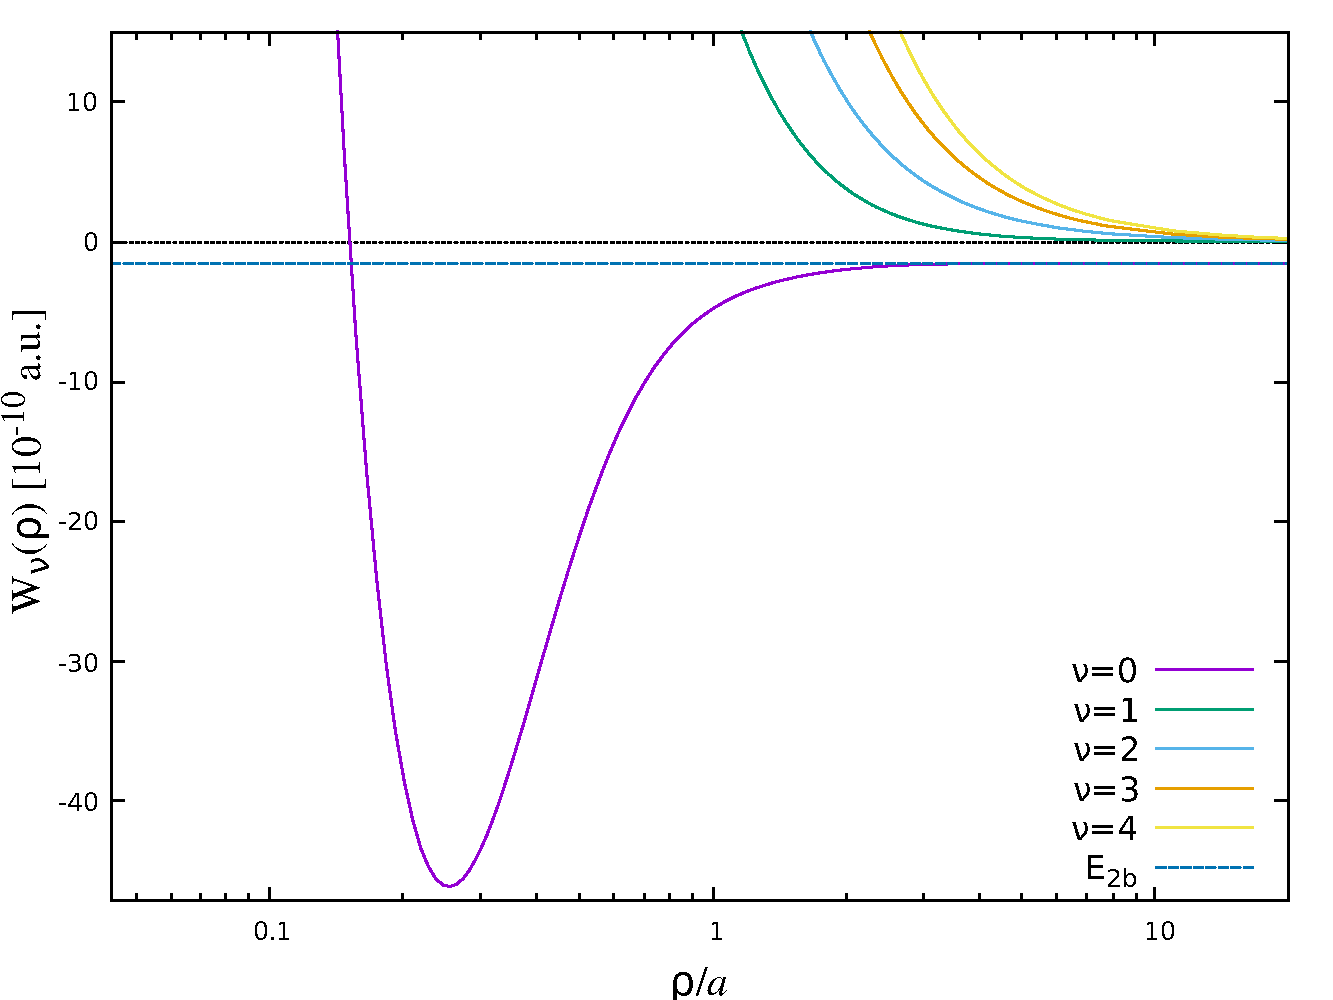
\includegraphics[width=1.0\linewidth]{Wpos.pdf}}
\end{columns}
\note[item]<1>{(The following discussion concerns short-ranged two-body interactions, where $|a| \gg r_0$)}
\note[item]<1>{The behavoiur of the 3-b potentials in the asymptotic limit, (i.e., when the hyperradius is much larger than the magnitude a) depend on the sign of a.}
\note[item]<2>{When a has a negative sign there is no weakly bound dimer and the lowest effective potential will converge to the three-body continuum channels, i.e., the kinetic energy for three free particles.}
\note[item]<4>{However, for systems of 3 identical bosons with a pair-wise attraction that is strong enough to support 2-body bound states, one 3-body effective potential curve will converge asymptotically to each two-body bound state.}
\end{frame}

\subsection{Intermediate Region}
\begin{frame}[label=W]
\frametitle{Convergence In the Intermediate Region}
	\visible<1->{\begin{block}{Intermediate Interaction Range}
\begin{equation*}
	r_0 \ll \rho \ll |a|
	\end{equation*}
\end{block}}
	
\visible<2->{\begin{block}{The Lowest Potential's Convergent Form (3 Identical Bosons)}
		\alert<3->{\begin{equation*}\label{eq:efimov_channel}
		W_{\nu}(\rho) = -\frac{s_0^2+\frac{1}{4}}{2\mu \rho^2}
		\end{equation*}} 
\end{block}}

\visible<4->{\begin{block}{Universal Constant (3 Identical Bosons)}
	\begin{equation*}
		s_0 \simeq 1.00624
	\end{equation*}
\end{block}}
\hyperlink{Results}{\beamerbutton{Jump to Results}}
\note[item]<1>{Efimov physics comes into play in the intermediate region.}
\note[item]<1>{In this region the three-body effective potentials are modified by the Efimov physics. It can lead to both attractive and repulsive effective potentials.}
\note[item]<2>{For 3 identical bosons the effective potential will be attractive and is responsible for the Efimov Effect!}
\note[item]<3>{And is responsible for the Efimov Effect!}
\note[item]<4>{The universal constant $s_0$ sets the size and energy scaling of succeding Efimov states.}
\end{frame}

%------------------------------------------------

\subsection{Analytical Model}
\begin{frame}[label=faddeev]
\frametitle{Analytic Model}
\begin{itemize}
\item<2->The adiabatic potentials $\nu_n$ can be determined analytically through the transcendental equation

\begin{equation*}
\sqrt{\nu_n} \cos{\bigg(\sqrt{\nu_n} \frac{\pi}{2}\bigg)} - \frac{8}{\sqrt{3}}\sin{\bigg(\sqrt{\nu_n} \frac{\pi}{6}\bigg)} = \sqrt{2}\alert<3>{\frac{\rho}{a}}\sin{\bigg(\sqrt{\nu_n} \frac{\pi}{2}\bigg)}
\end{equation*}

\item<4-> Three-body effective potential $$W_{\nu}(\rho/a)=\frac{(\nu_n(\rho/a)-\frac{1}{4})}{2\mu \rho^2}$$
\end{itemize}
\hyperlink{R_faddeev}{\beamerbutton{Jump to Results}}
\note[item]<1>{We can obtain a similair result analytically by instead of solving the SE we solve the coupled Faddeev equations}
\note[item]<2>{We then obtain the adiabatic potential $\nu$ through the transcendental eq.}
\note[item]<3>{This adiabatic potential is a function of $\rho/a$}
\note[item]<4>{It is related to the 3-body potential}
\note[item]<4>{In the result section I will compare these solutions to my numerically calculated potentials.}
\end{frame}

%------------------------------------------------

\section{Numerical Approach}
\begin{frame}{Numerical Approach; B-spline Collocation}
\only<1>{ 
	\centering
	\huge
	Task = ?}
\only<2>{ 
	\centering
	\huge
	Task = Find \alert<2>{$W_{\nu}(\rho)$}!}
\invisible<-2>{
\parallelcontent
{\begin{description} \item<3->[First:] Choose a basis \end{description}}
{\begin{itemize}\item<4->$\varphi_{lm} = \varphi_{1l}(\theta)\varphi_{2m}(\phi)$\end{itemize}}
\parallelcontent
{\begin{description} \item<5->[Then:] Expand \end{description}}
{\begin{itemize}\item<6->$\Phi_{\nu}(\rho;\theta,\phi) = \sum_{l,m}^{L,M} c_{lm}\varphi_{lm}$\end{itemize}}
\parallelcontent
{\begin{description} \item<7->[Next:] Substitute $\Phi_{\nu}$ into the
		\hyperlink<7->{supplemental}{\beamerbutton{Adiabatic Eq.}
		\hypertarget<7->{matrix}}  \end{description}}
{\begin{itemize}\item<8->$\mathbf{H}_{\mathrm{ad}}\mathbf{c} = U\mathbf{B}\mathbf{c}$\end{itemize}}
\parallelcontent
{\begin{description} \item<9->[Finally:] Solve the Generalized Eigenvalue Eq. \end{description}}
{\begin{itemize}\item<10->$W(\rho) \approx U(\rho)$\end{itemize}}}
\note[item]<1>{So what what was task?}
\note[item]<2>{Well, a good start is to find the 3-b effective potentials}
\note[item]<3>{To do this I have choosen two work with a B-spline basis for the two angular coordinates}
\note[item]<4>{We expand the solutions in this basis}
\note[item]<5>{And put it into the adiabatic eq.}
\note[item]<6>{And finally solve the Generalized eigenvalue eq.}
\end{frame}

%------------------------------------------------
\section{Scattering Model}
\begin{frame}
\frametitle{Scattering Model}
\begin{columns}
	\column{0.4\textwidth}
\begin{block}<1->{Masses} 
	$m = m(Rubidium-87)$
\end{block}
\begin{block}<2->{Assumption}
	$V(\rho,\theta,\psi) = v(r_{12}) + v(r_{23}) + v(r_{31})$
\end{block}
\begin{block}<3->{2B Model Potential}
	$v(r) = d\cosh^{-2}{(r/r_0)}$
\end{block}
\begin{block}<4->{Interaction Range}
	$r_0 = 55$ a.u.
\end{block}
\column{0.6\textwidth}
\only<3->{
%\begin{figure}
	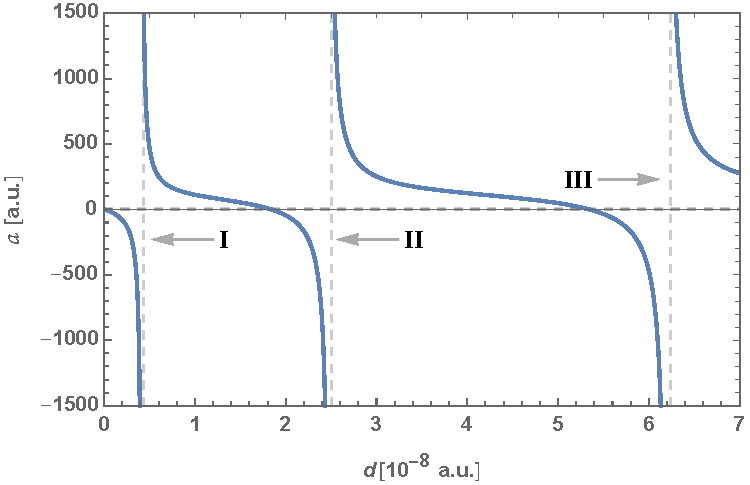
\includegraphics[width=1.0\linewidth]{scattering_new.pdf}}
%\end{figure}
\end{columns}
\note[item]<1>{For the scattering model I have used masses corresponding to Rb-87 (boson)(Z=37, N=50)}
\note[item]<2>{I have used the assumption that the total potential can be written as a sum of 2-b potentials}
\note[item]<3>{I have used the following model potential because I can calculate the scattering length from it}
\note[item]<4>{And set the interaction range to 55 a.u.}
\end{frame}
%------------------------------------------------

\section{Results}
\subsection{Convergence and Accuracy}
\begin{frame}
\frametitle{Convergence and Accuracy}
\begin{itemize}
	\item<1->{
	\hypertarget{Results}
	For $a \rightarrow \pm \infty$ we expect convergence towards
	\hyperlink{W}{\beamerbutton{the Efimovian form}}}
	\item<2-> Easier to recognize if the potentials are multiplied by $2 \mu \rho^2$ and plotted as 
	
	\begin{equation*}
	\xi(\rho) = 2 \mu \rho^2 W_{\nu}(\rho) + \frac{1}{4}
	\end{equation*}
	\item<3-> Should approach the universal value $-s_0^2 (\simeq -1.0125$) in the intermediate region
\end{itemize}
\vfill
\hyperlink{finite}{\beamerbutton{To Figures}}
\note<1>{And now to the results!}
\note<1>{For $a \rightarrow \pm \infty$ we expect that the lowest effective potential curve will converge towards the Efimovian form}
\note<2>{This behaviour is easier to recognize if the potentials are multiplied by this factor $2 \mu \rho^2$ and plot them as}
\note<2>{Since these curves should approach the universal value $-s_0^2 (\simeq -1.0125$) in the intermediate region}
\end{frame}

\begin{frame}[label=finite]
\frametitle{Efimov-like Potentials $\xi(\rho)$ for Different $a$}
	\vspace*{-0.6cm}
	\begin{columns}[t]
	\column{0.5\textwidth}
	\only<1>{
	\centering
	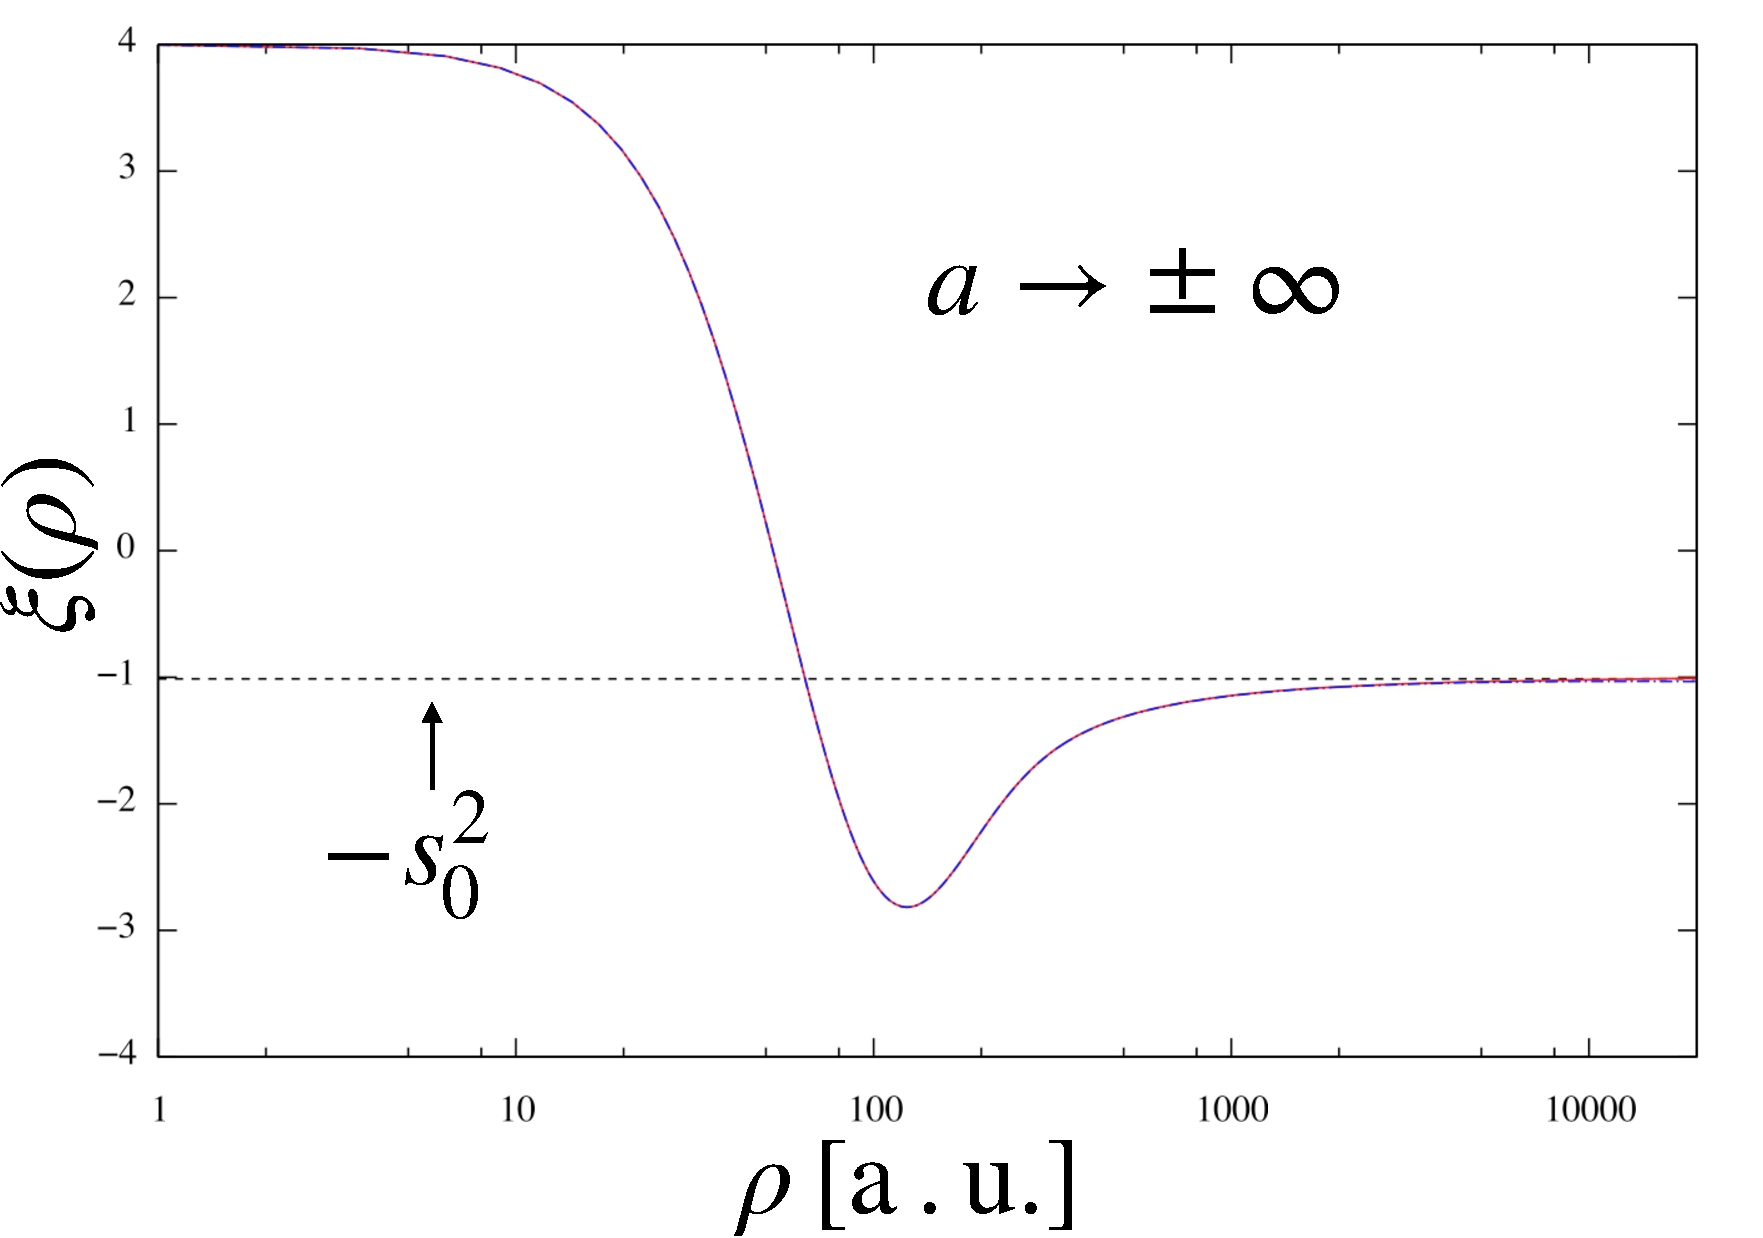
\includegraphics[width=1.0\linewidth]{infty_p.pdf}}
	\only<2-5>{
	\centering
	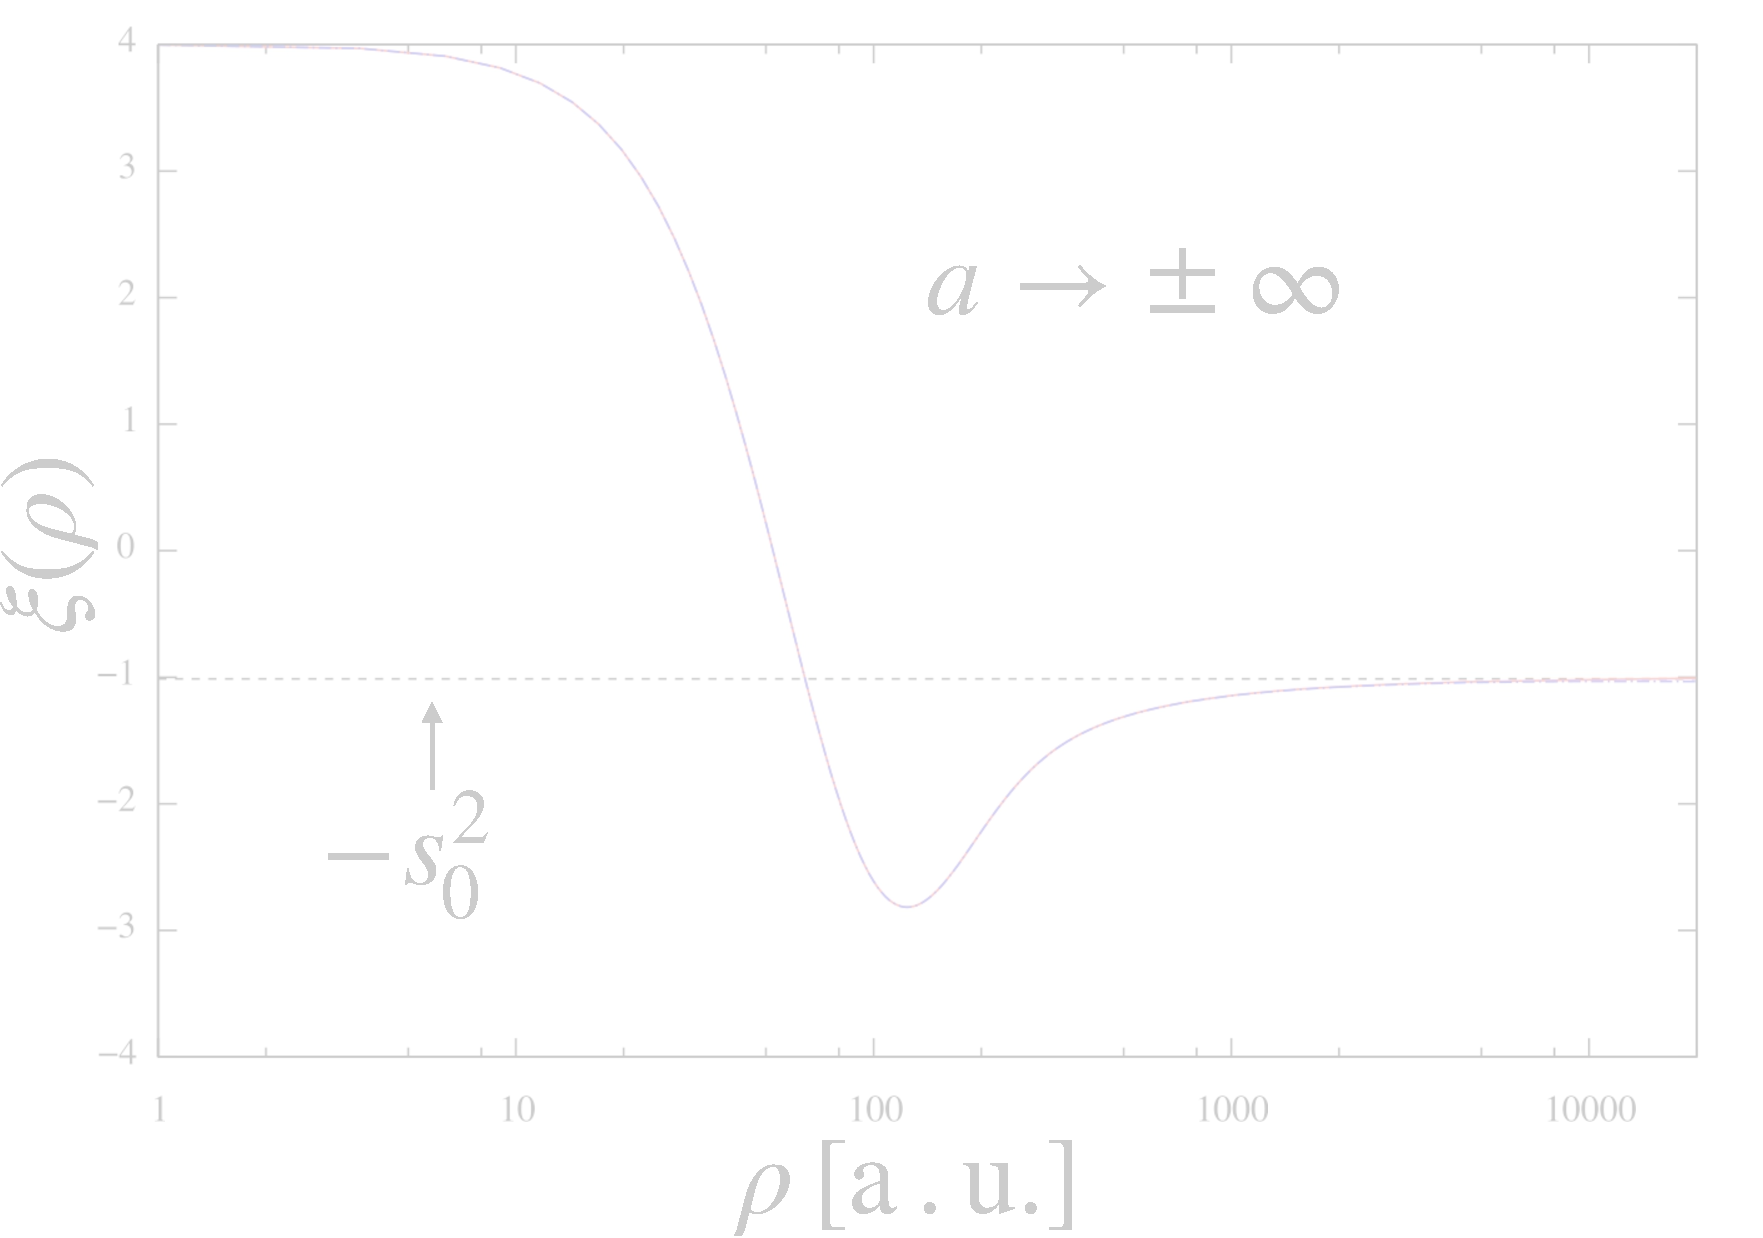
\includegraphics[width=1.0\linewidth]{infty_opac.pdf}}
	\only<1-2,5>{
	\centering
	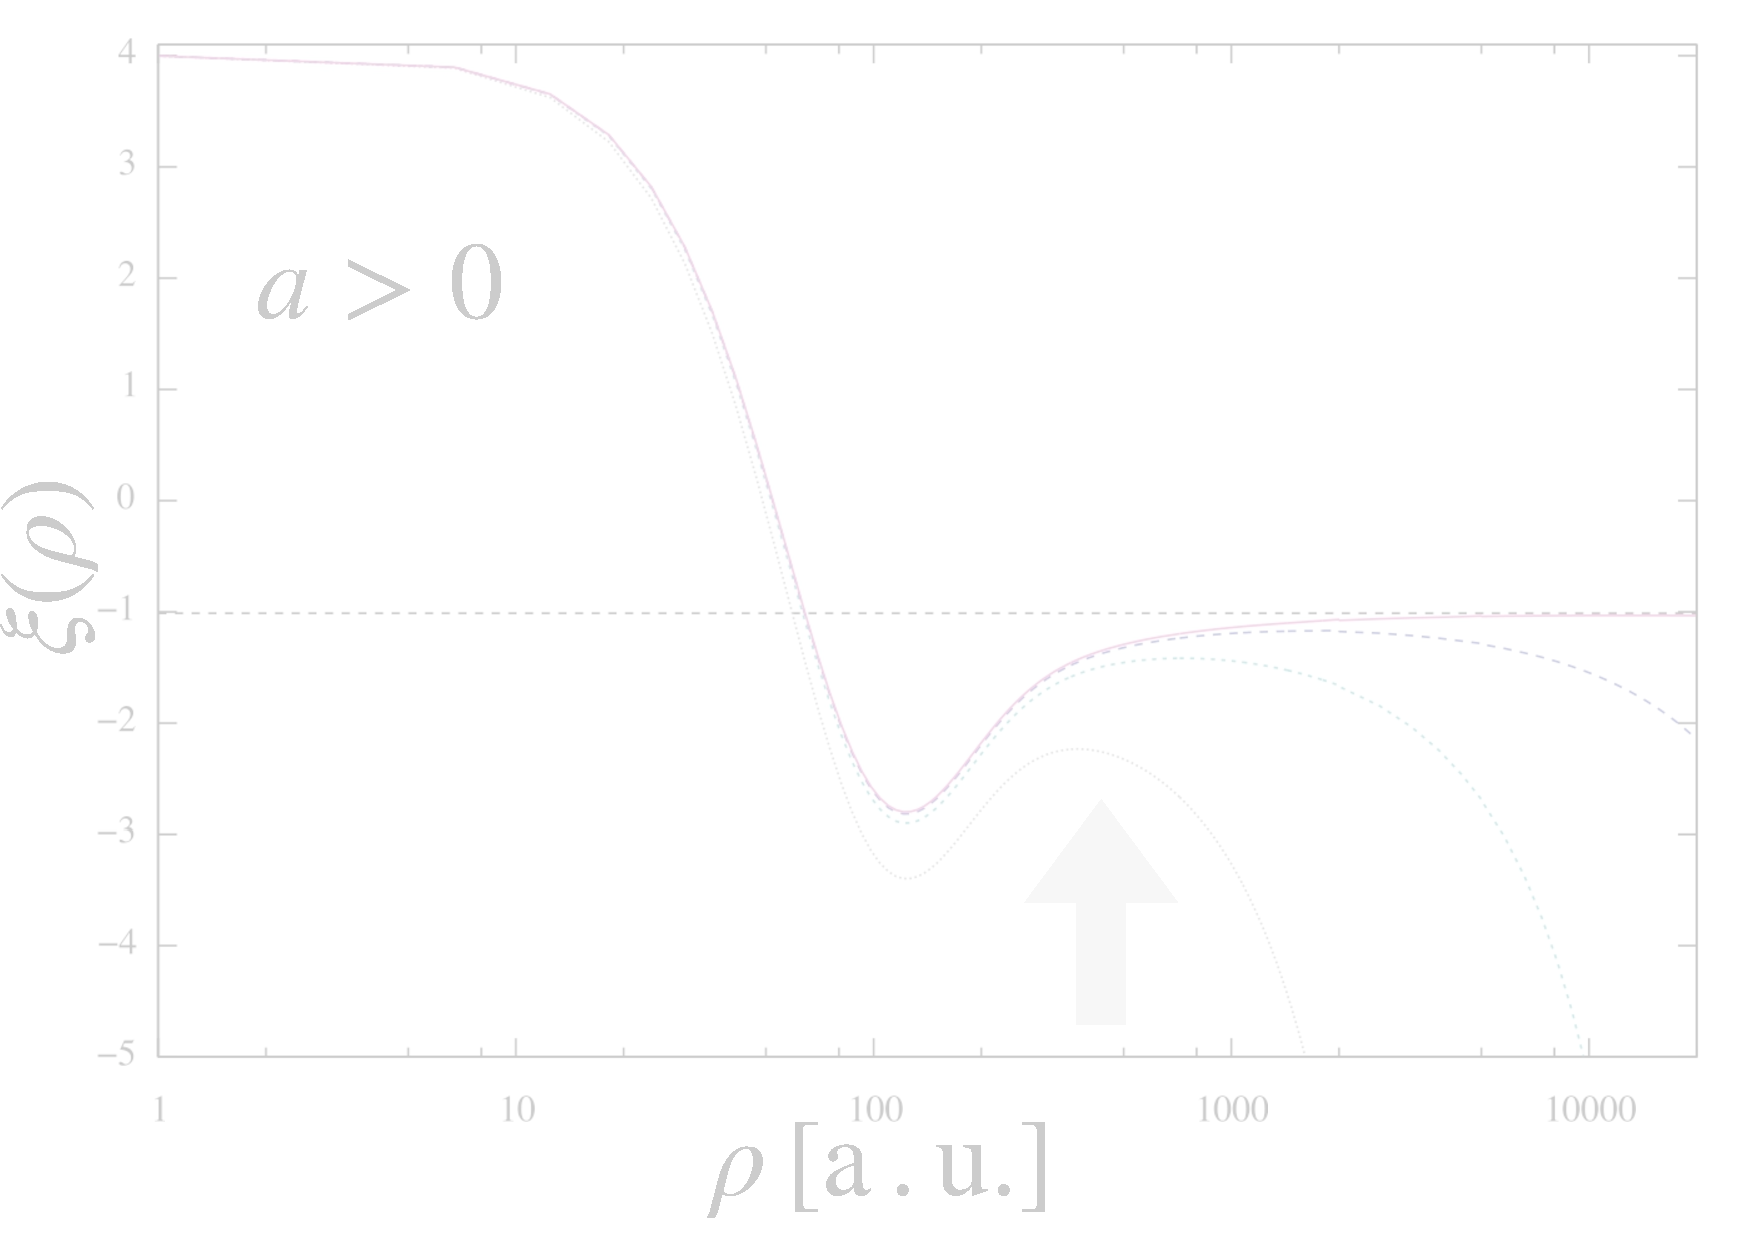
\includegraphics[width=1.0\linewidth]{finite_positive_opac.pdf}}
	\only<3-4>{
	\centering
	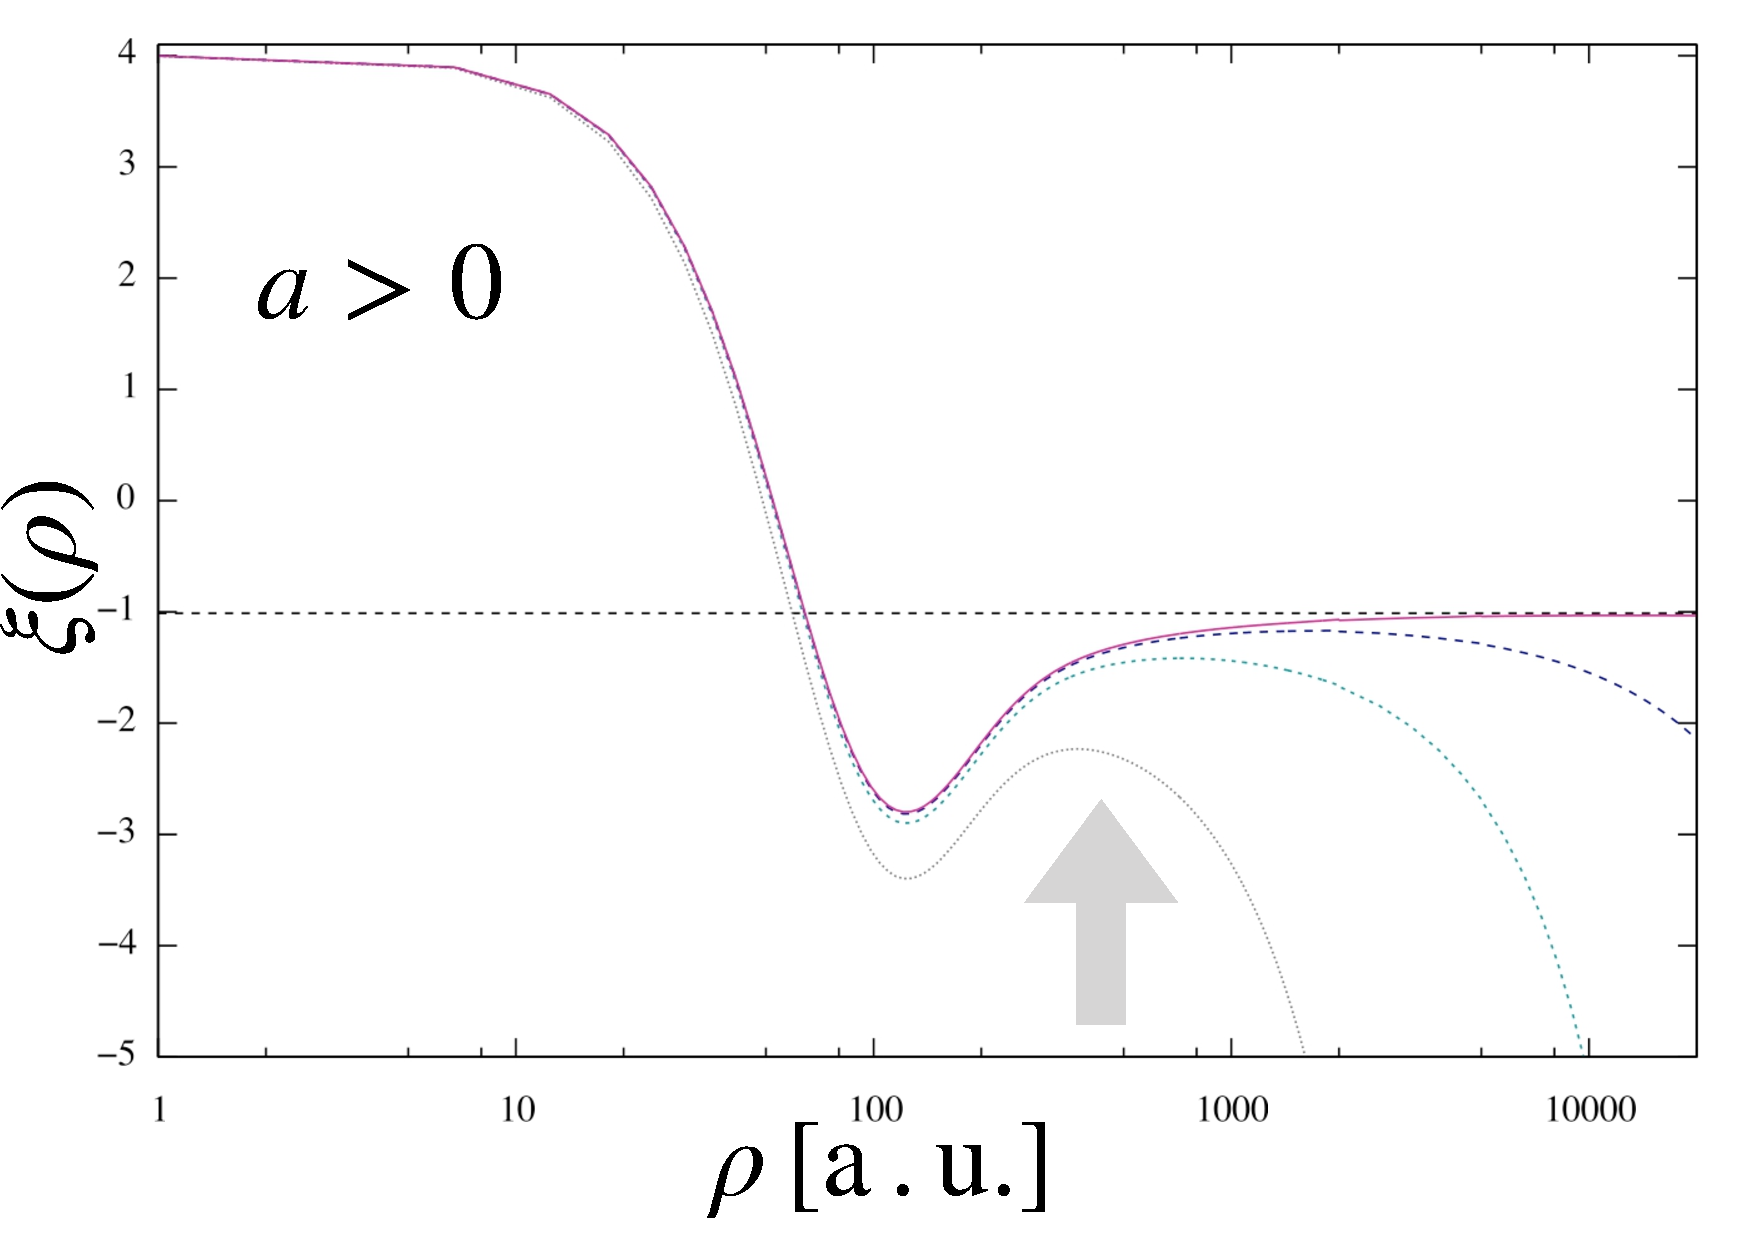
\includegraphics[width=1.0\linewidth]{finite_positive_p.pdf}}
	\column{0.5\textwidth} %New column
	\only<1,3-5>{
	\centering
	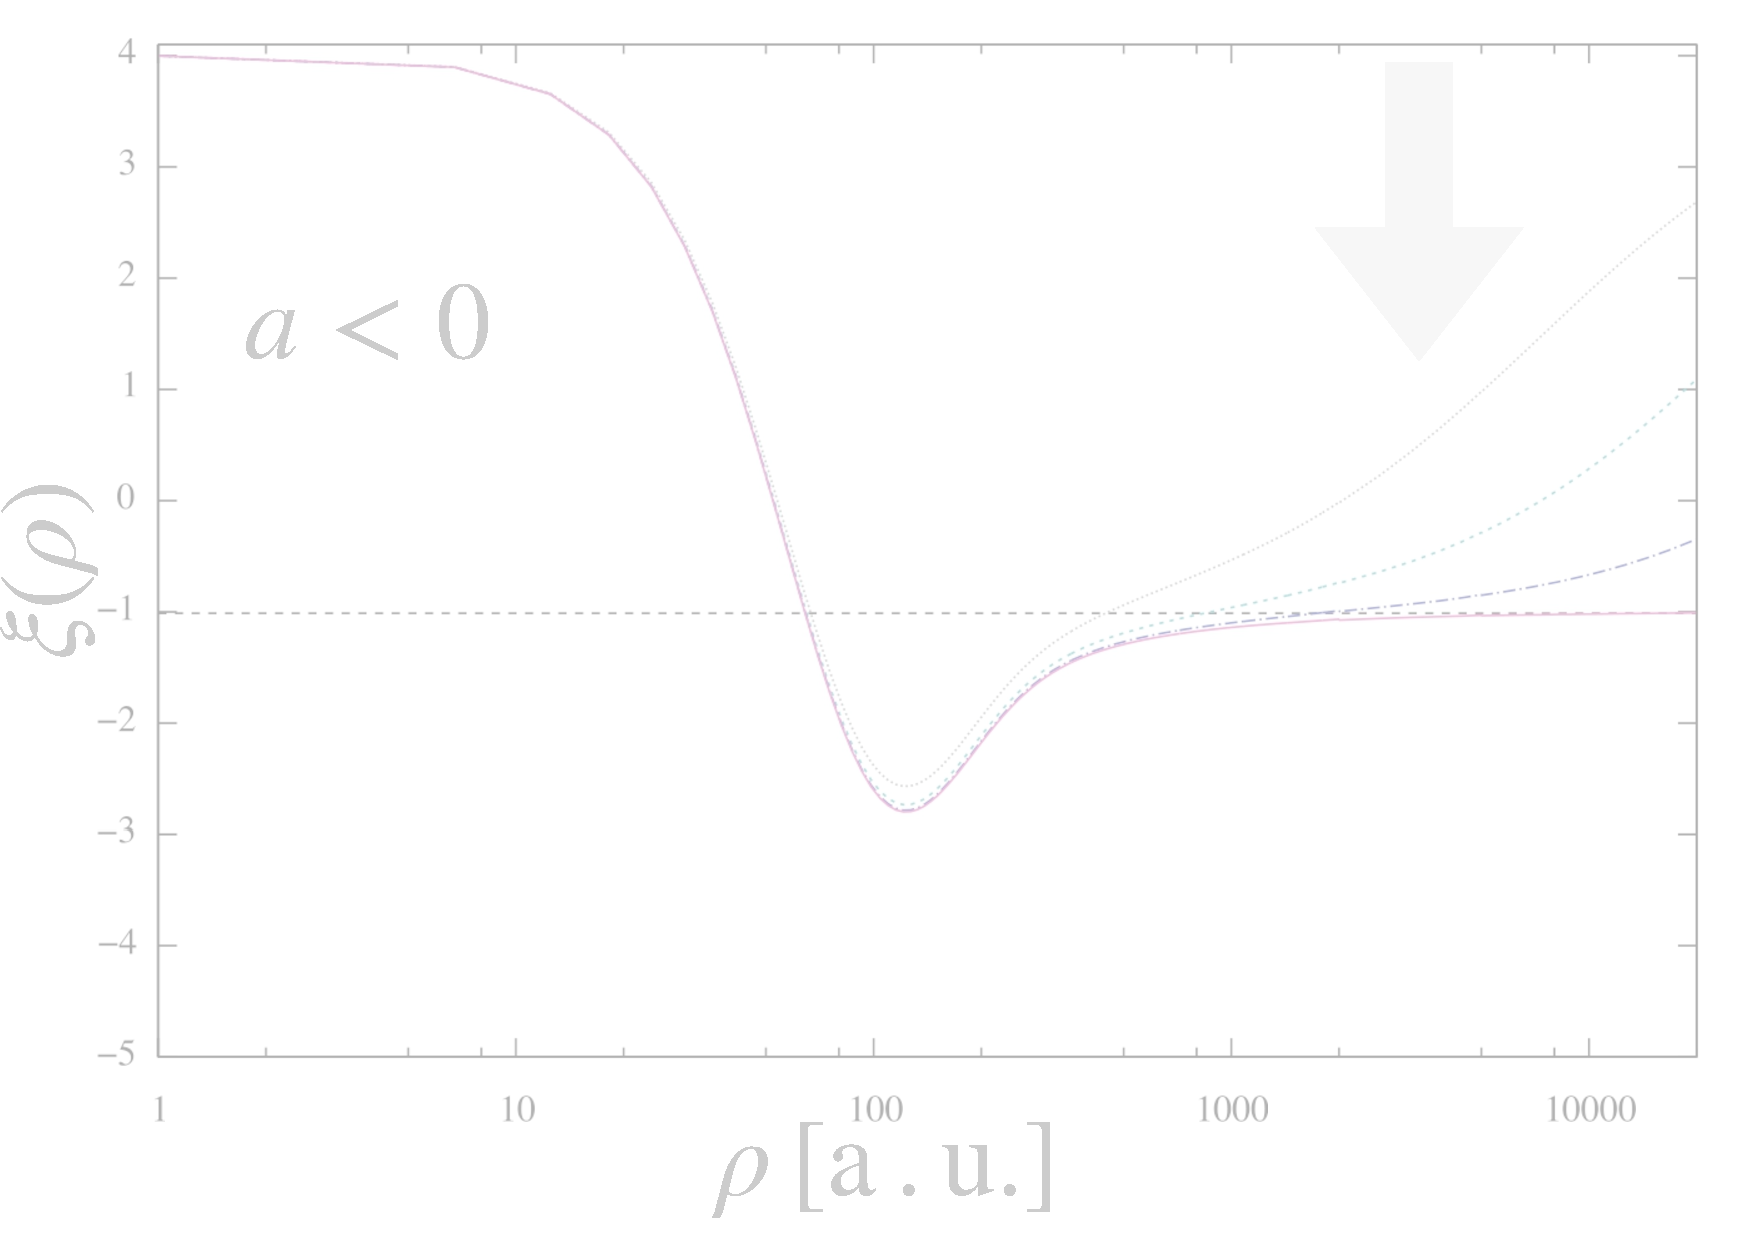
\includegraphics[width=1.0\linewidth]{finite_negative_opac.pdf}}
	\only<2>{
	\centering
	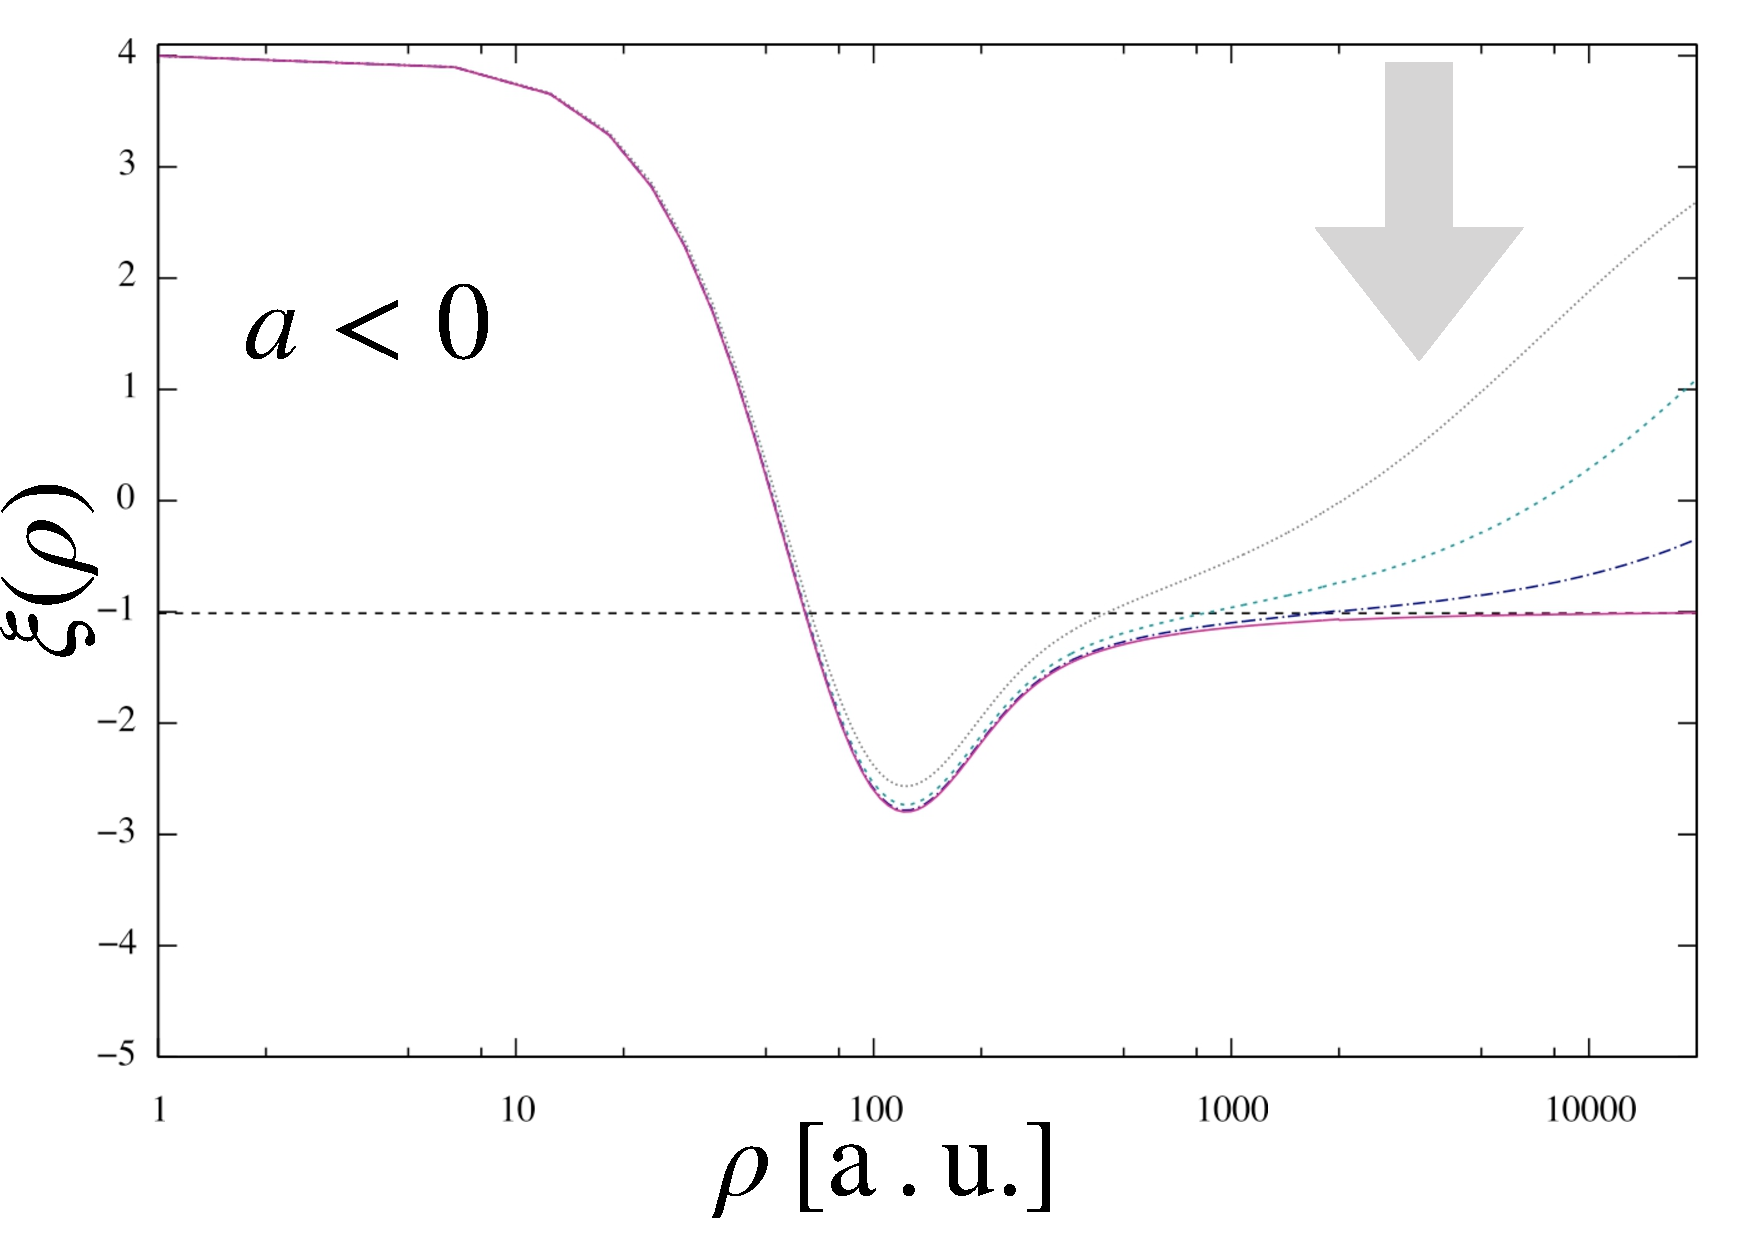
\includegraphics[width=1.0\linewidth]{finite_negative_p.pdf}}
	\only<4>{
	\centering
	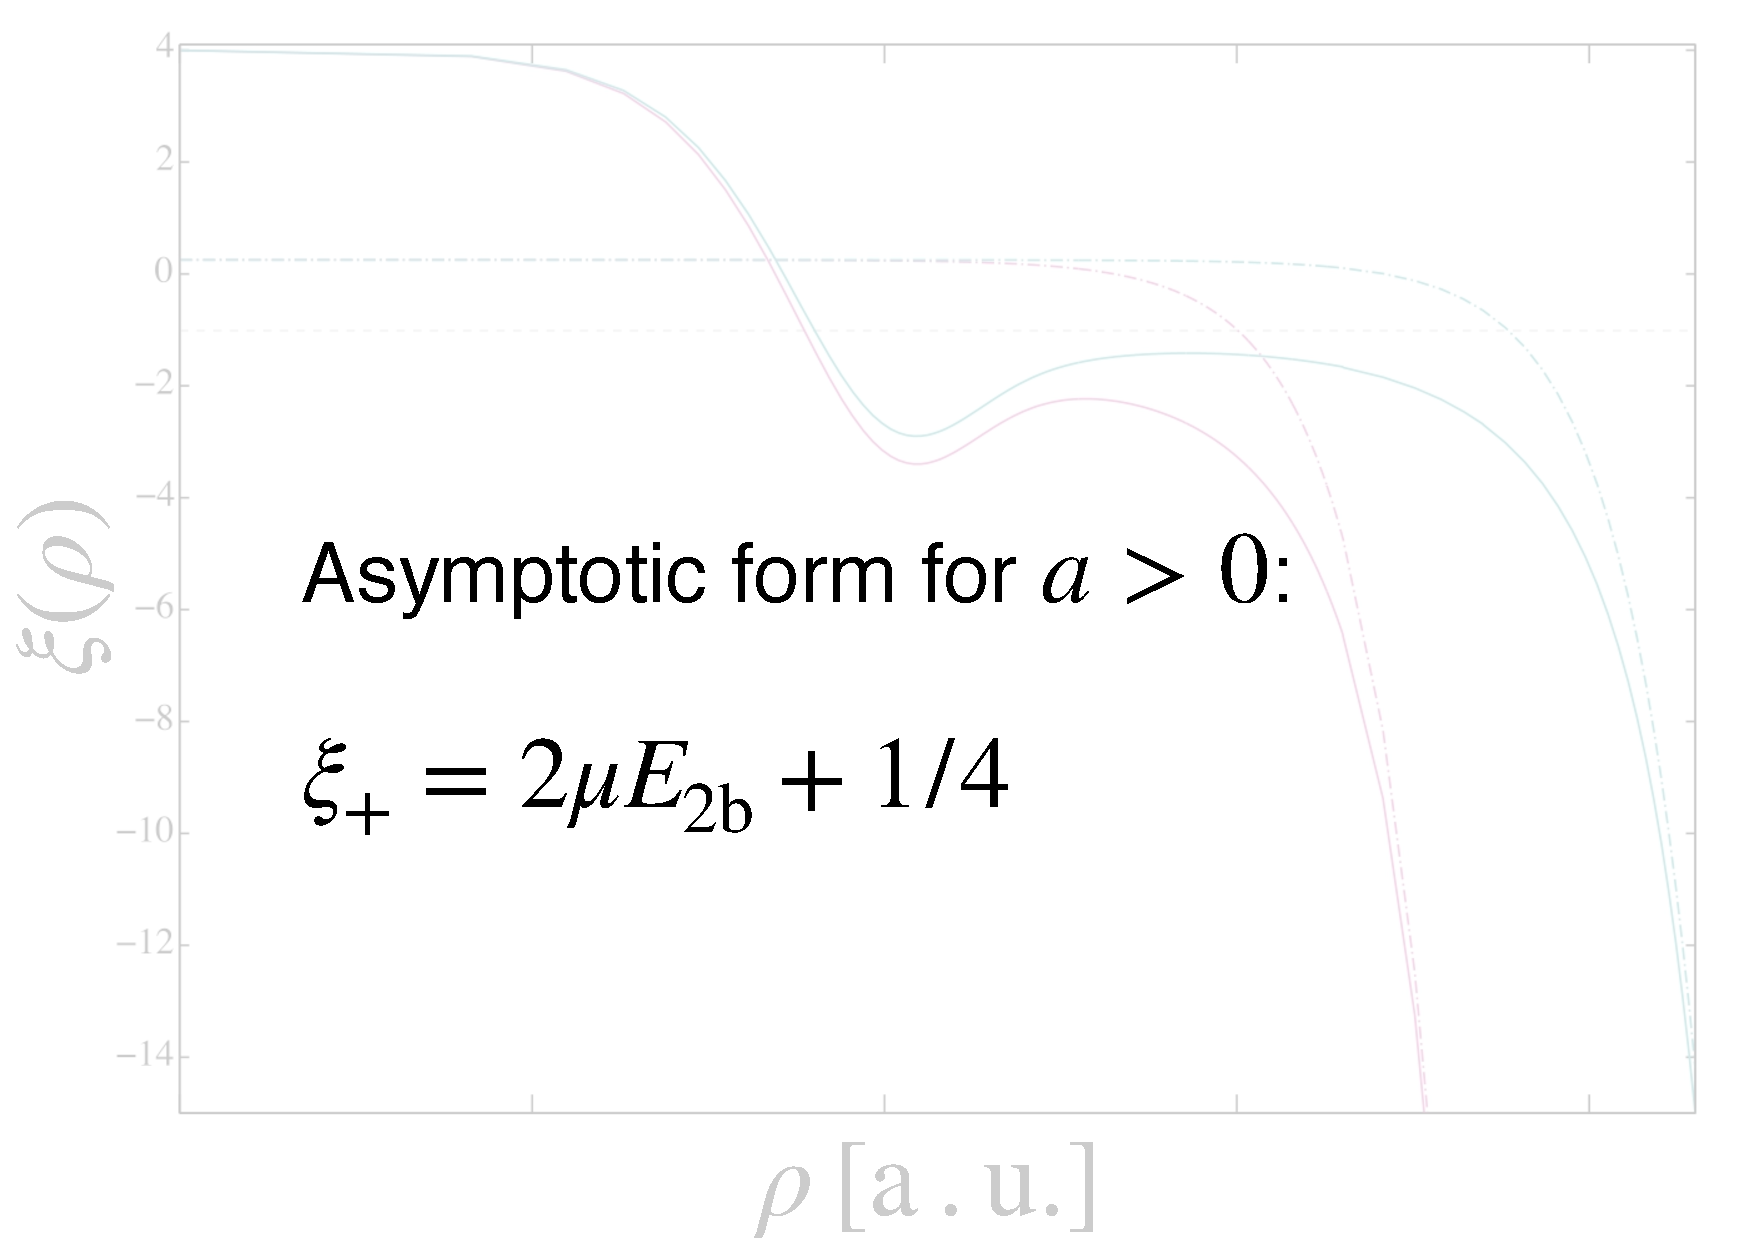
\includegraphics[width=.97\linewidth]{finite_conv_asym.pdf}}
	\only<5>{
	\centering
	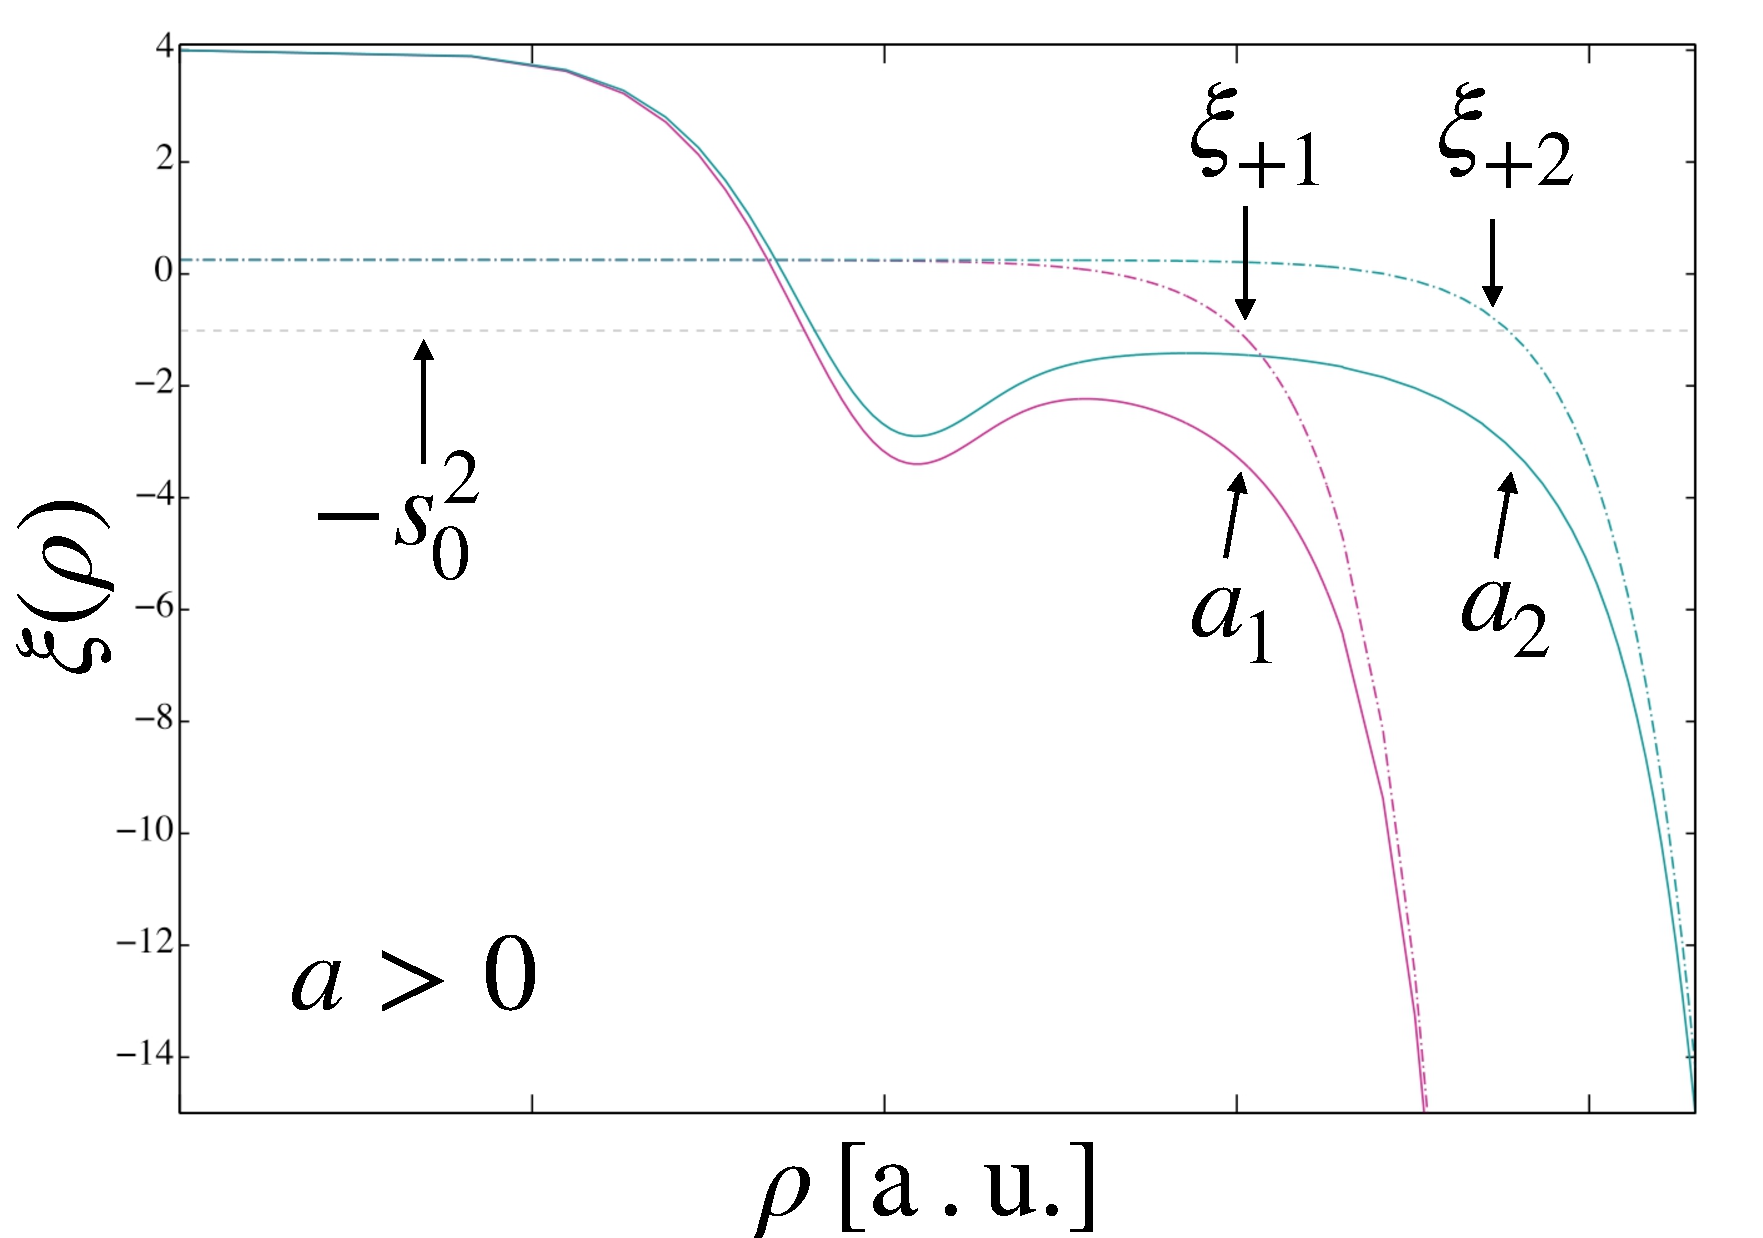
\includegraphics[width=1.0\linewidth]{finite_conv_p.pdf}}
	\only<1-3>{
	\centering
	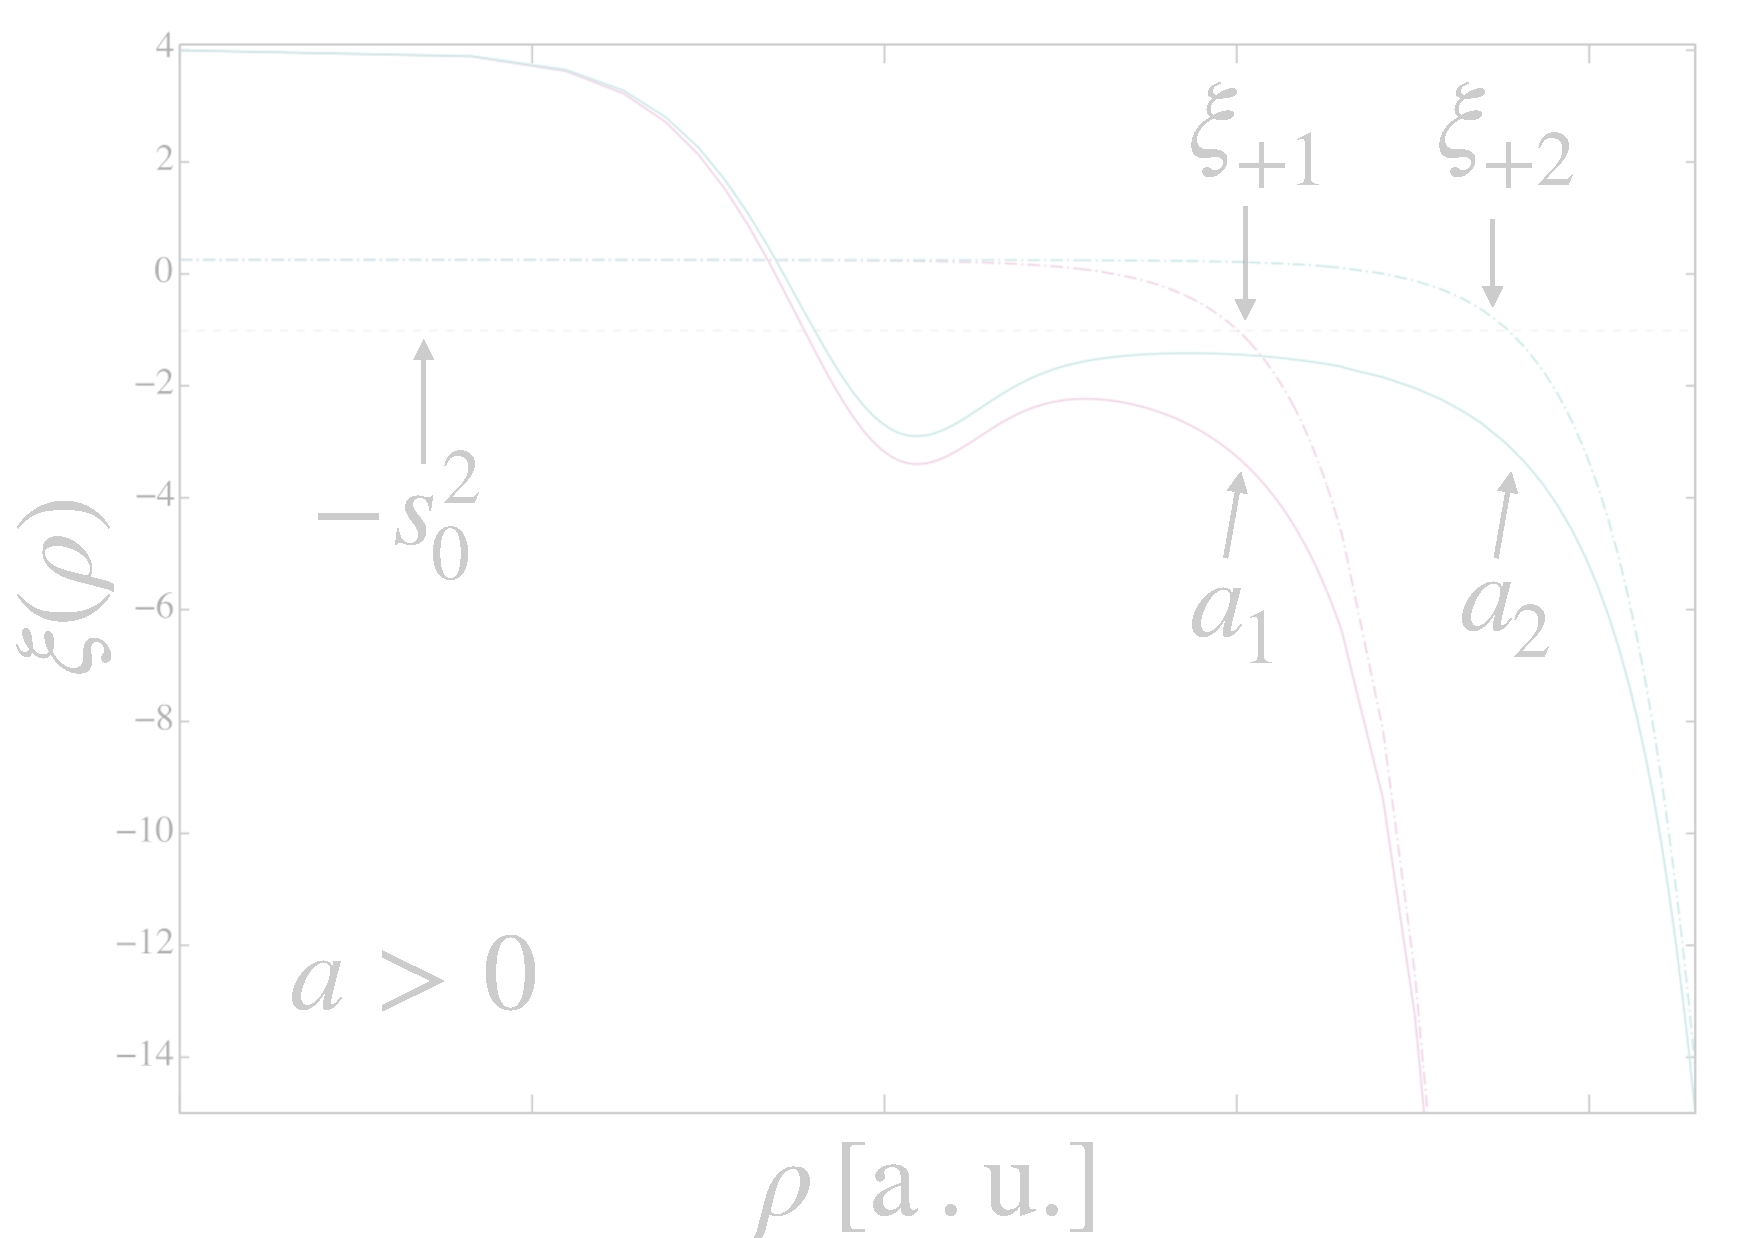
\includegraphics[width=1.0\linewidth]{finite_conv_opac.pdf}}
	\end{columns}
\hyperlink{asymptotic}{\beamerbutton{Effective Potentials}}
\hyperlink{Results}{\beamerbutton{$\xi(\rho)$}}
\note[item]<1>{When the scattering length diverge we see that the potential curve $\xi$ converge to the expected value at large hyperradii (note the log scale on the $\rho$-axis)}
\note[item]<1>{For two-body potentials where $|a|$ is large but finite we expect that the effective potentials are to some extent affected by Efimov physics in the intermediate range ($r_0 \ll \rho \ll |a|$) and that the lowest effective potentials obtained with a larger magnitude of a exhibit closer resemblance with the true Efimov potential}
\note[item]<2>{This is indeead what we see for negative $a$. Here I have plotted 4 curves with $|a|$ ranging from 2000 to 3 M a.u. (the curves start to converge to the kinetic energy in the asymptotic limit)}
\note[item]<3>{This is also the case for large positive $a$. We see a flattening behaviour of the curves from below which tend to get closer to the universal value as $a$ increase.However, here the curves will start to converge to the energy of the two body bound state. Here I have plotted 4 curves with $|a|$ ranging from 2000 to 3 M a.u. (the curves start to converge to the kinetic energy in the asymptotic limit)}
\note[item]<4>{However, in this case the curves will start to converge to the energy of the two body bound state. Which here corresponds to}
\note[item]<5>{Here I have plotted the two curves with lowest $a$ together with the curves $\xi$ corresponding to the 2-b energies and we observe that the curves indeed converge to the 2-b energy in the asymptotic limit.}
\end{frame}

%--------------------------------------------------------------------------------------

\subsection{Comparison to the Analytical Model}
\begin{frame}[label=R_faddeev]
\frametitle{Comparison to the Analytical Model (1)}
	\only<1>{
	\centering
	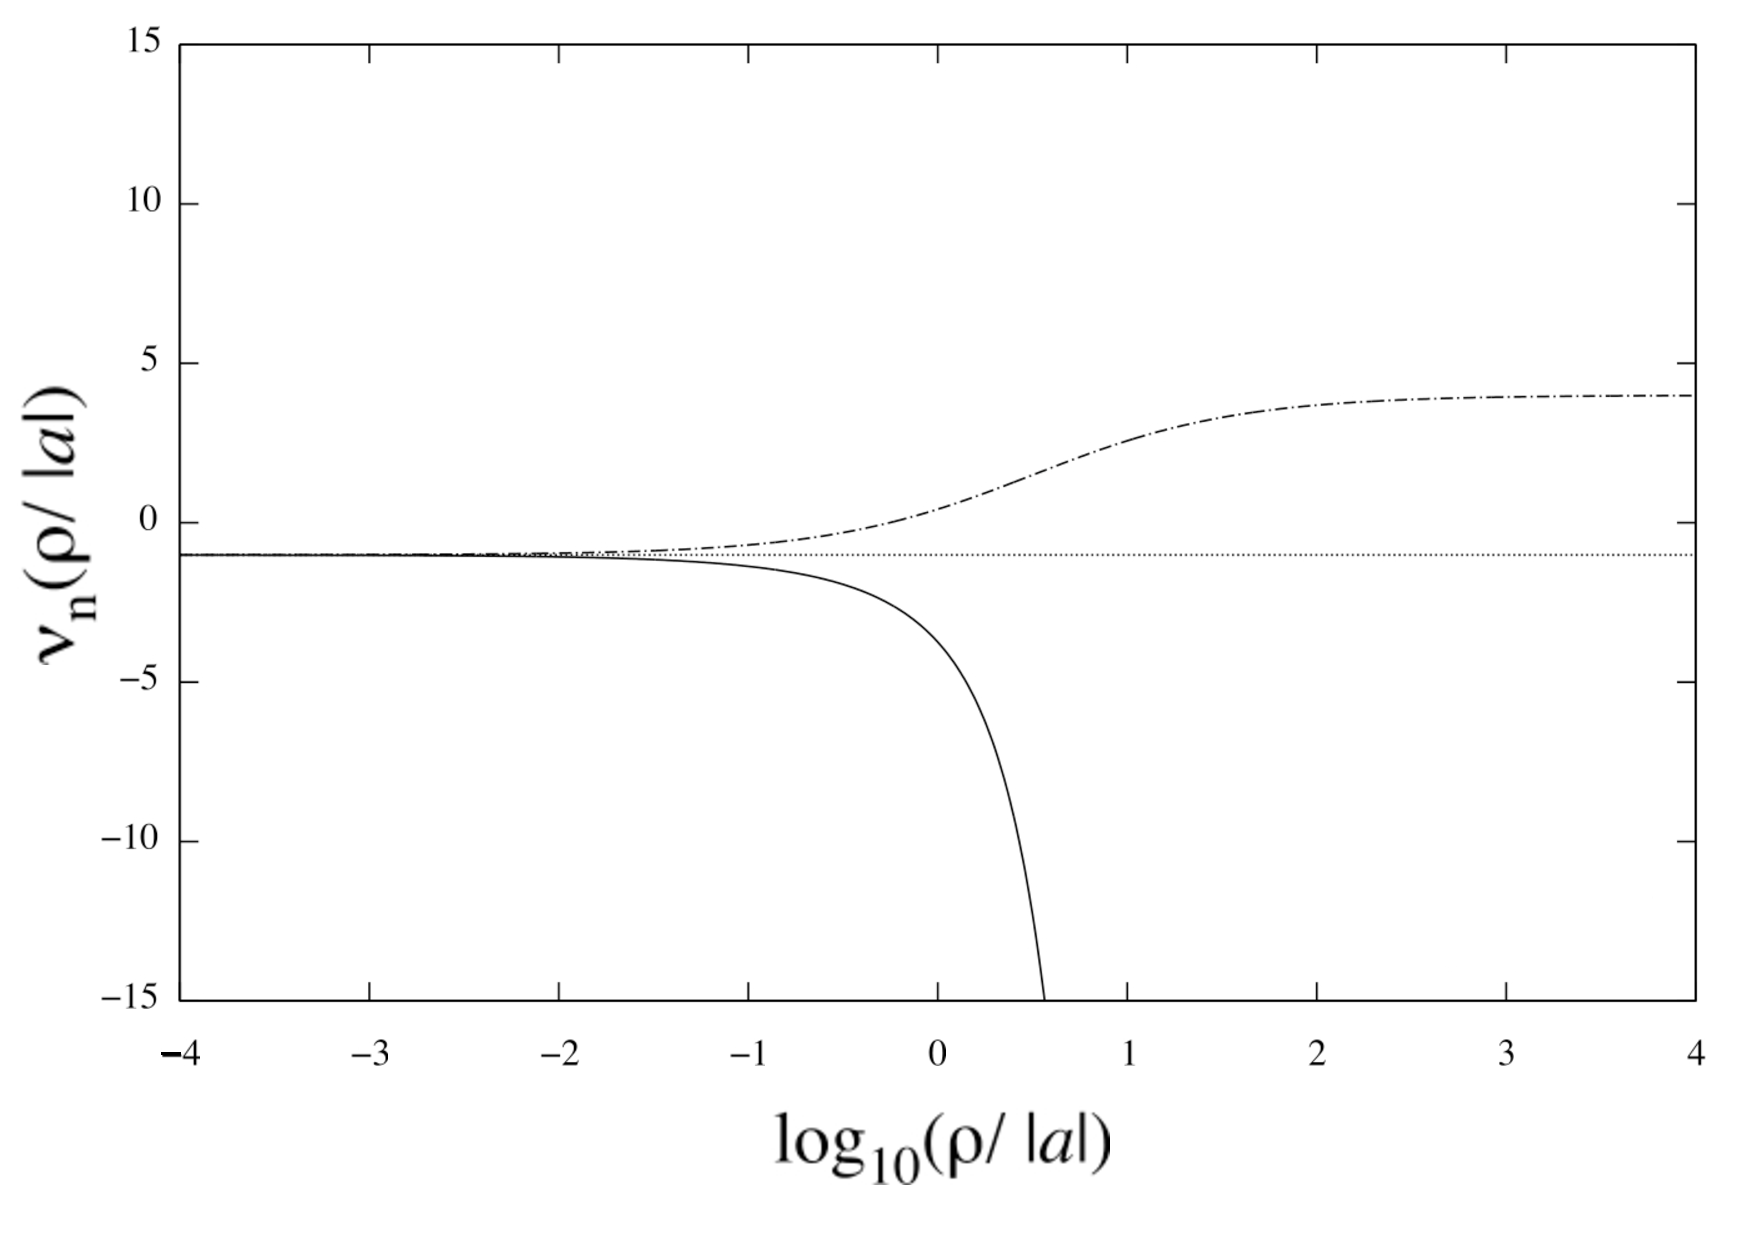
\includegraphics[width=1.0\linewidth]{faddeev0.pdf}}
	\only<2>{
	\centering
	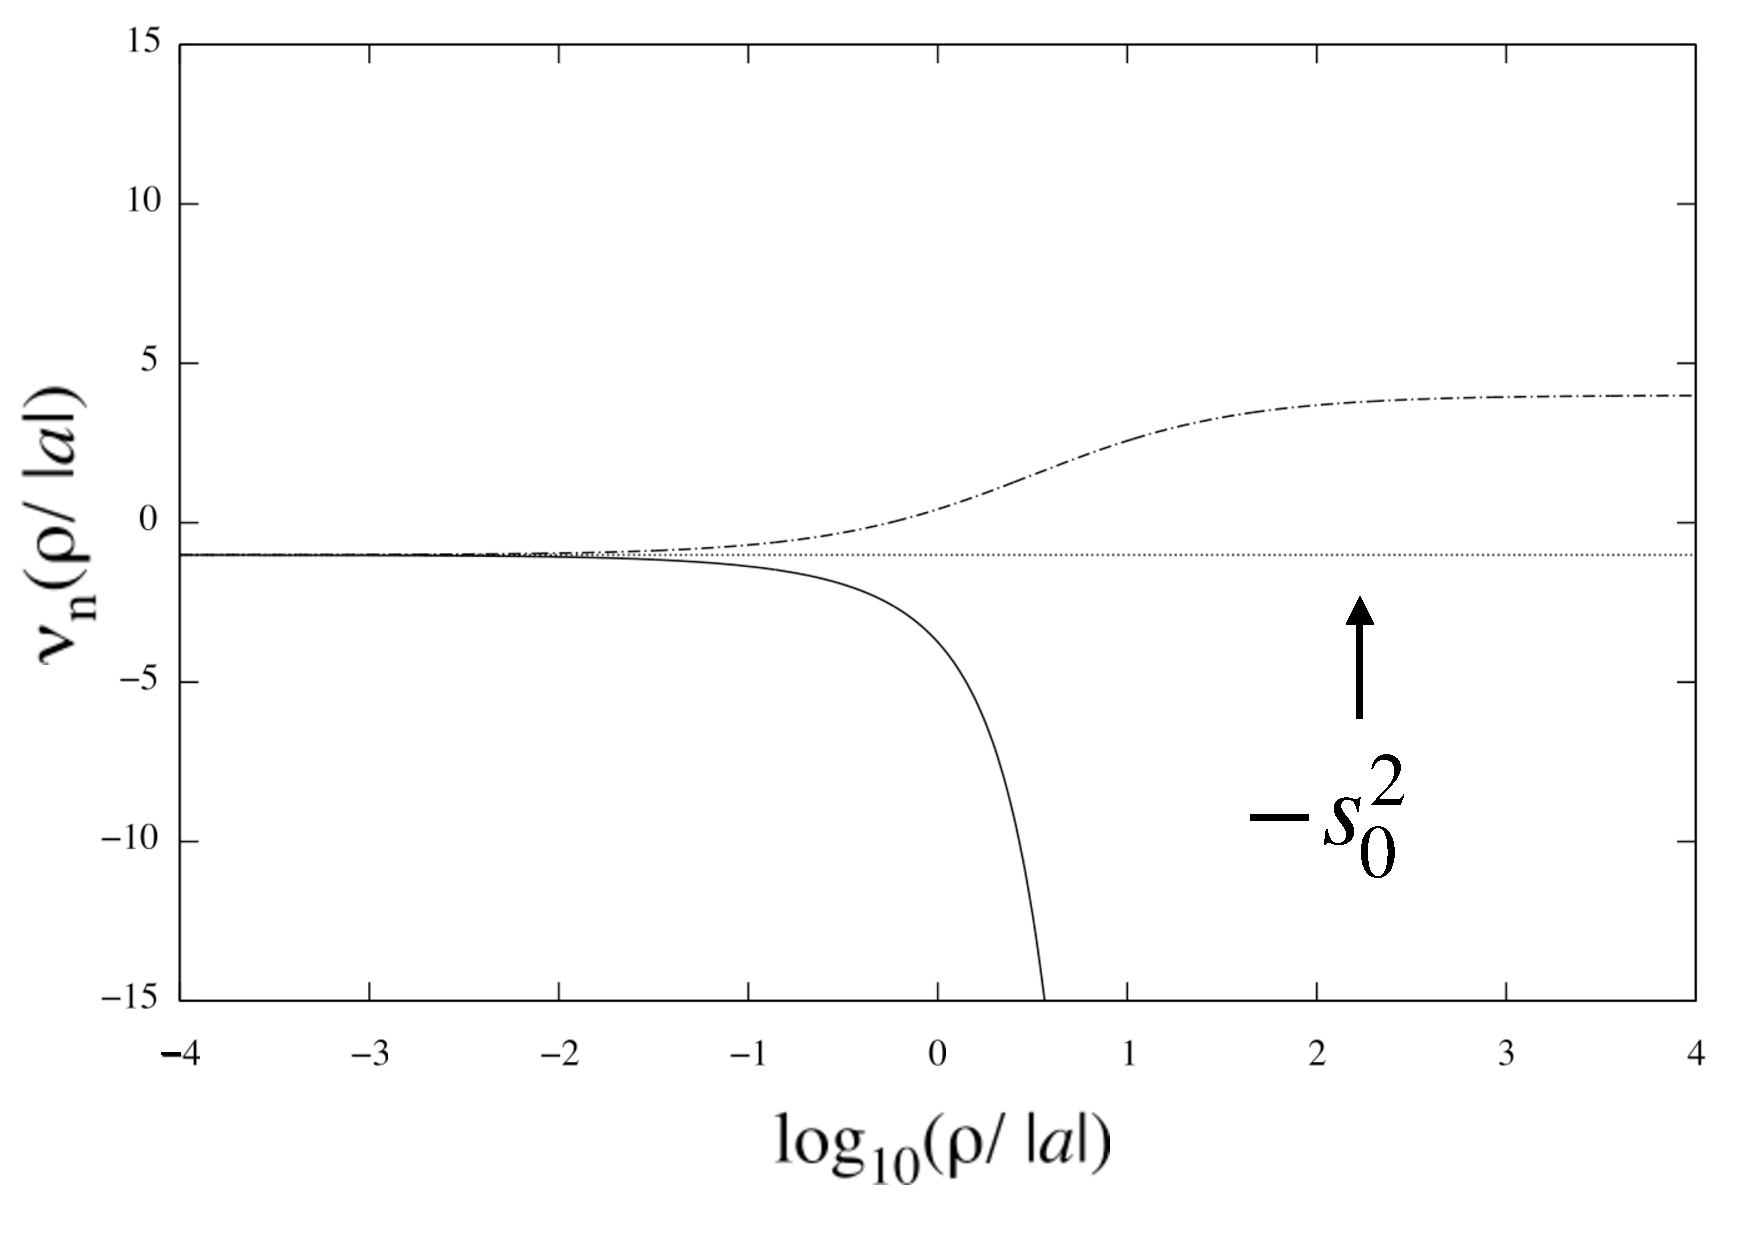
\includegraphics[width=1.0\linewidth]{faddeev1.pdf}}
	\only<3>{
	\centering
	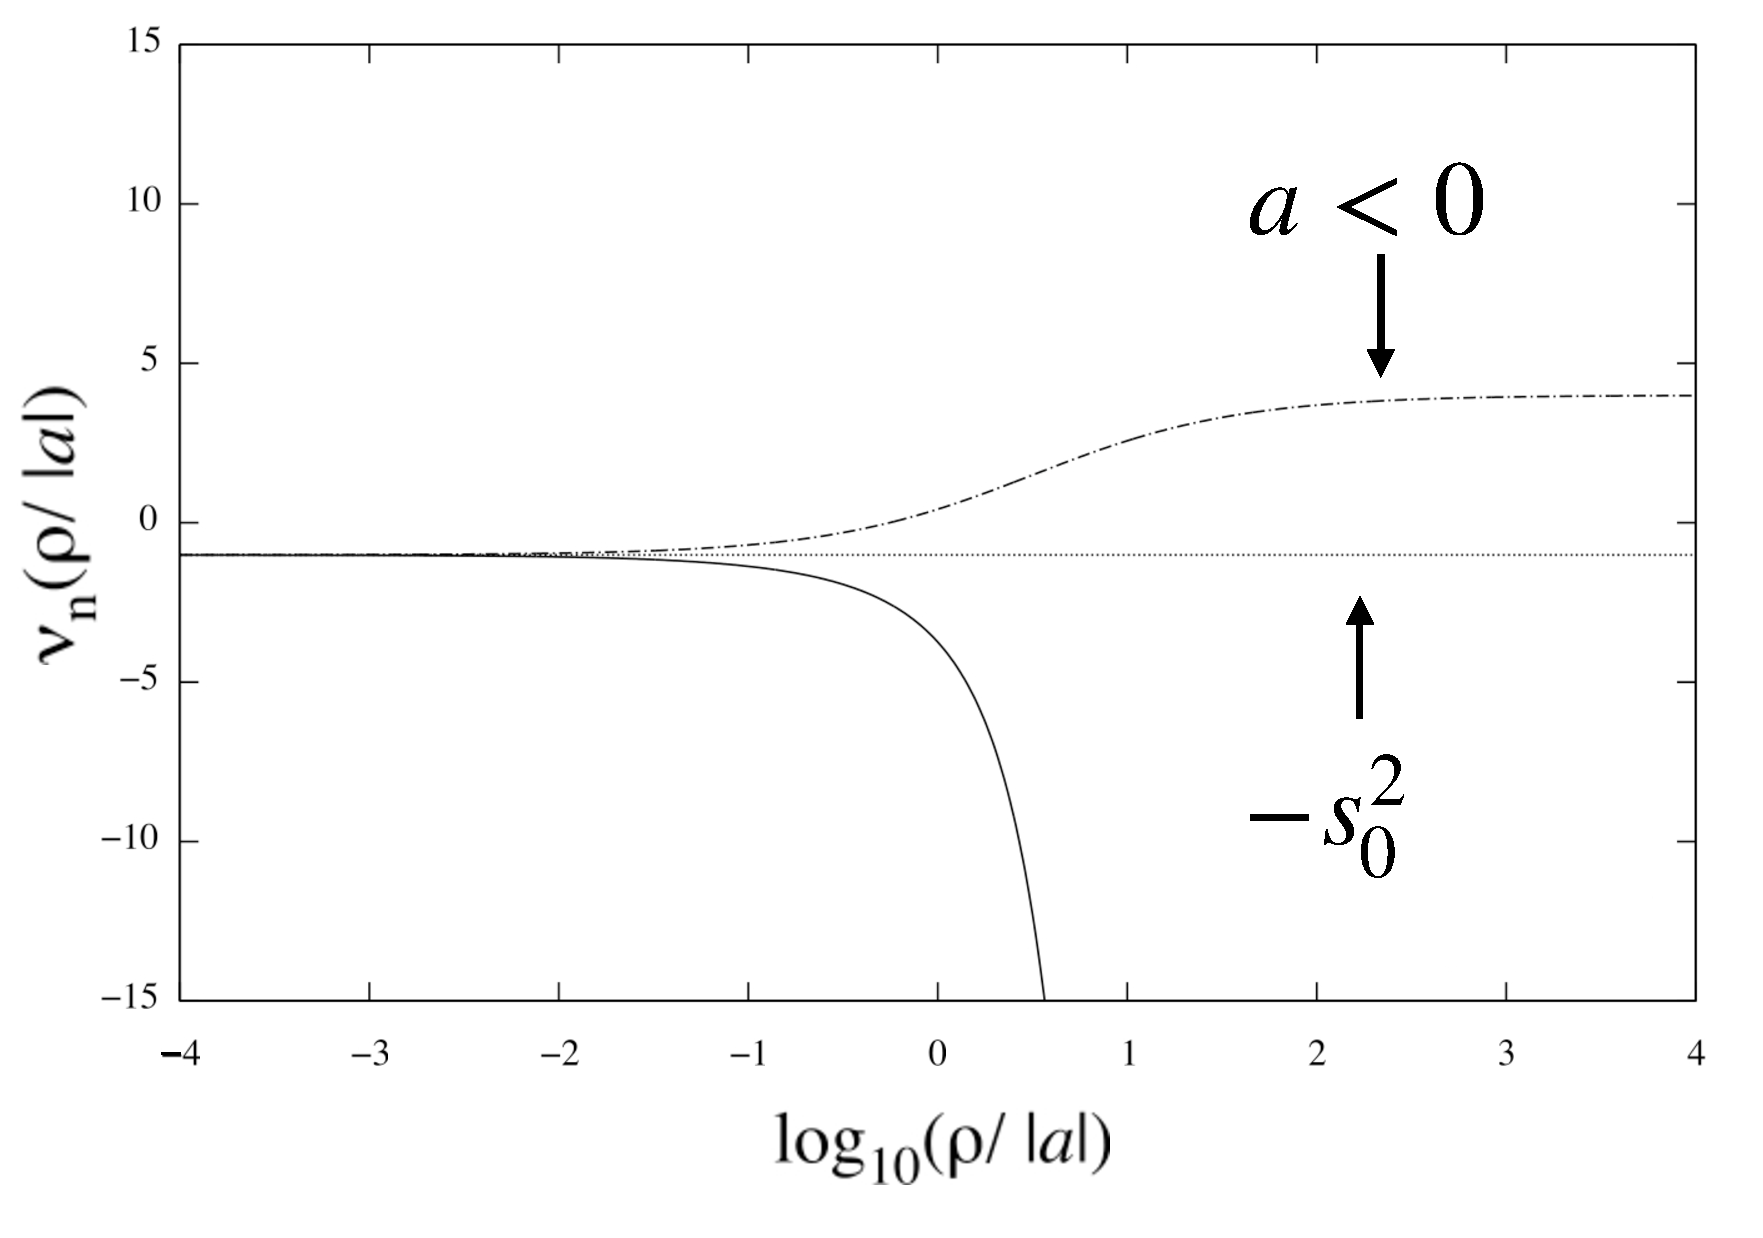
\includegraphics[width=1.0\linewidth]{faddeev2.pdf}}
	\only<4>{
	\centering
	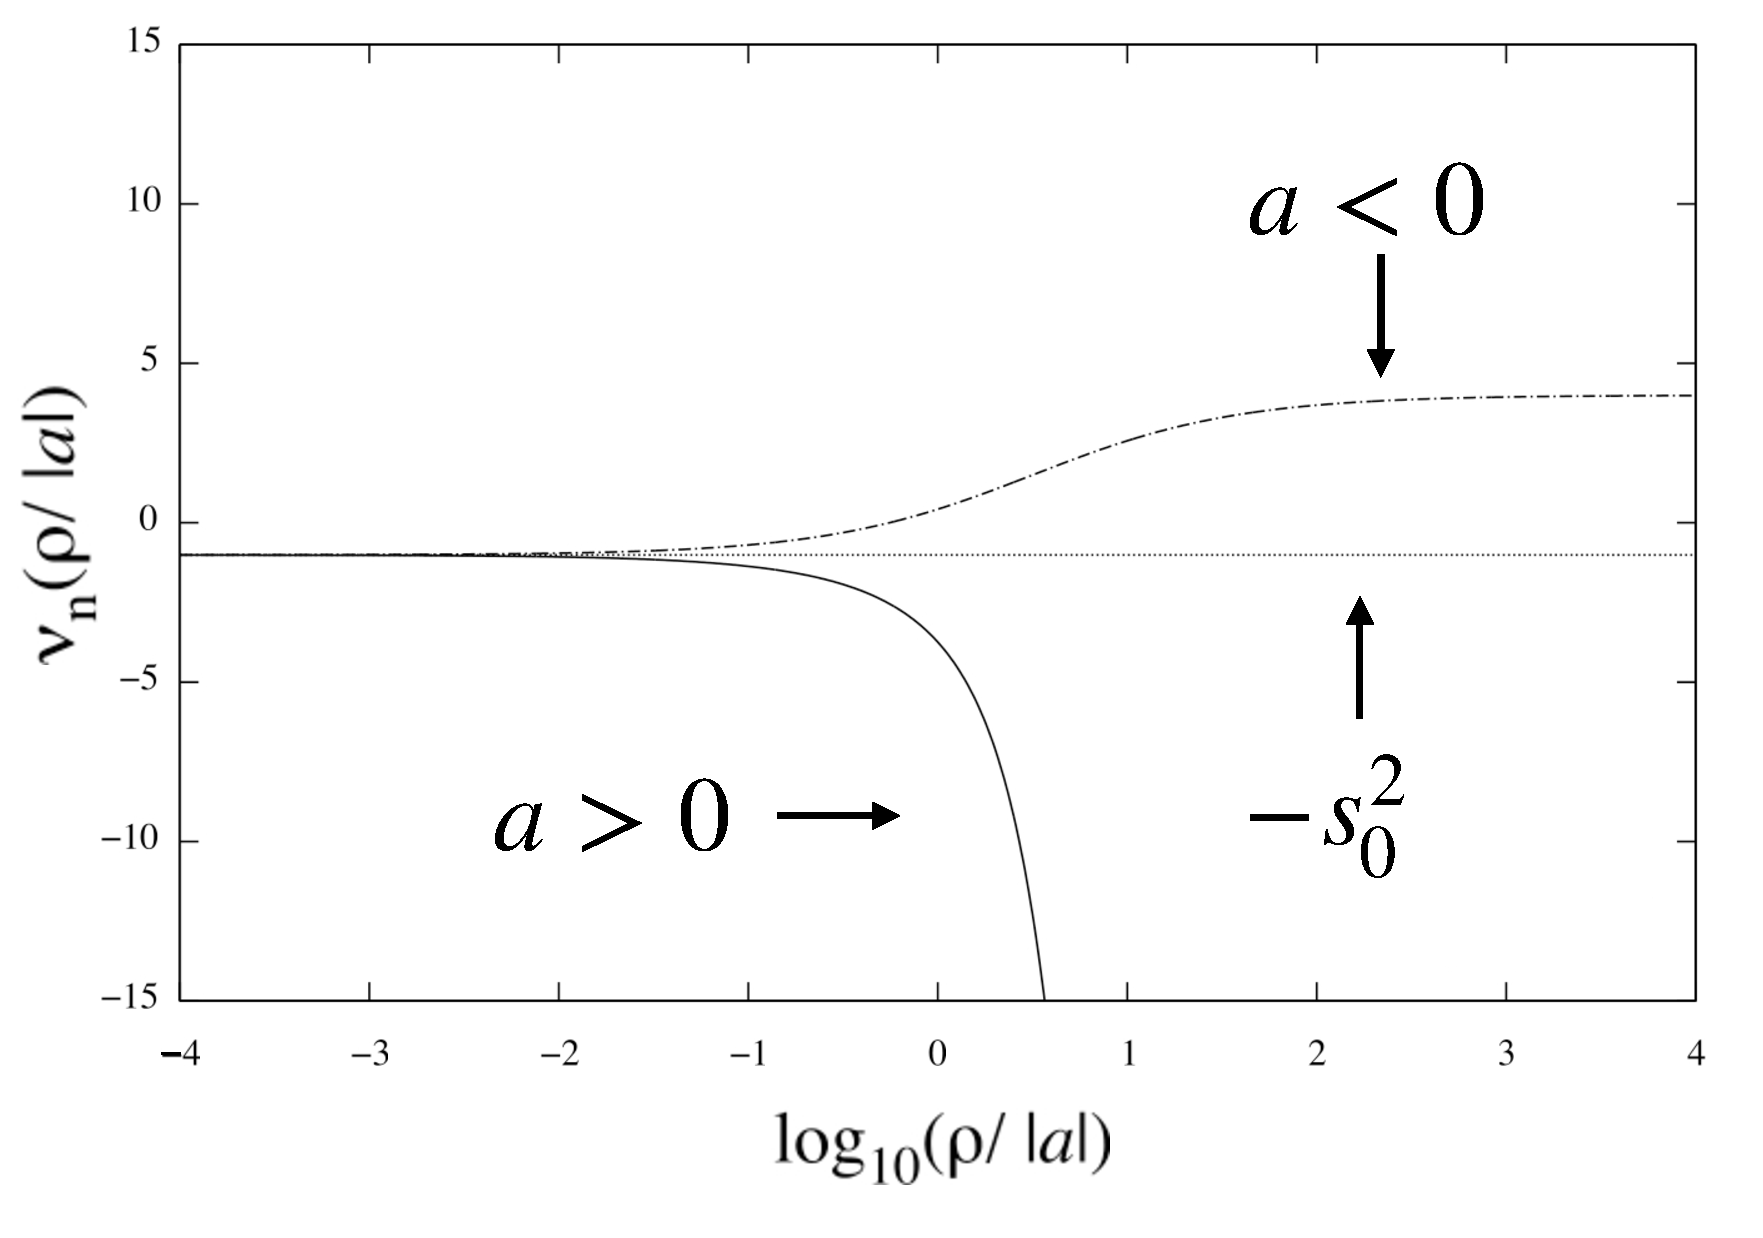
\includegraphics[width=1.0\linewidth]{faddeev3.pdf}}
\visible<1-4>{
\begin{textblock*}{9cm}(0mm,1.15\textheight)
		\hyperlink{faddeev}{\beamerreturnbutton{Analytic Potential}}
		\hyperlink{neg2}{\beamergotobutton{$a<0$}}
		\hyperlink{pos1}{\beamergotobutton{$a>0$}}         
\end{textblock*}}
%\hyperlink{faddeev}{\beamerbutton{Faddeev}}
\note[item]<1>{With this figure I want to show the equivalent lowest potentials for positive and negative $a$ calculated from the transcendental Faddeev eq.}
\note[item]<2>{The universal value is shown as a this dotted line. And we can se that when $a>\rho$, the adiabatic potential for both positive and negative $a$ converge to this universal value.}
\note[item]<3>{When $\rho>|a|$ we can observe that the curve for negative $a$ approach the value corresponding to the kinetic energy for three particles.}
\note[item]<4>{For postive $a$, we intead observe a parabolic behaviour like that corresponding to the form of the energy of the 2-b bound state when $\rho>a$.}
\end{frame}

\begin{frame}
\frametitle{Comparison to the Analytical Model (2)}
	\only<1>{
	\centering
	\vspace*{0.0cm}
	\hspace*{-0.2cm}
	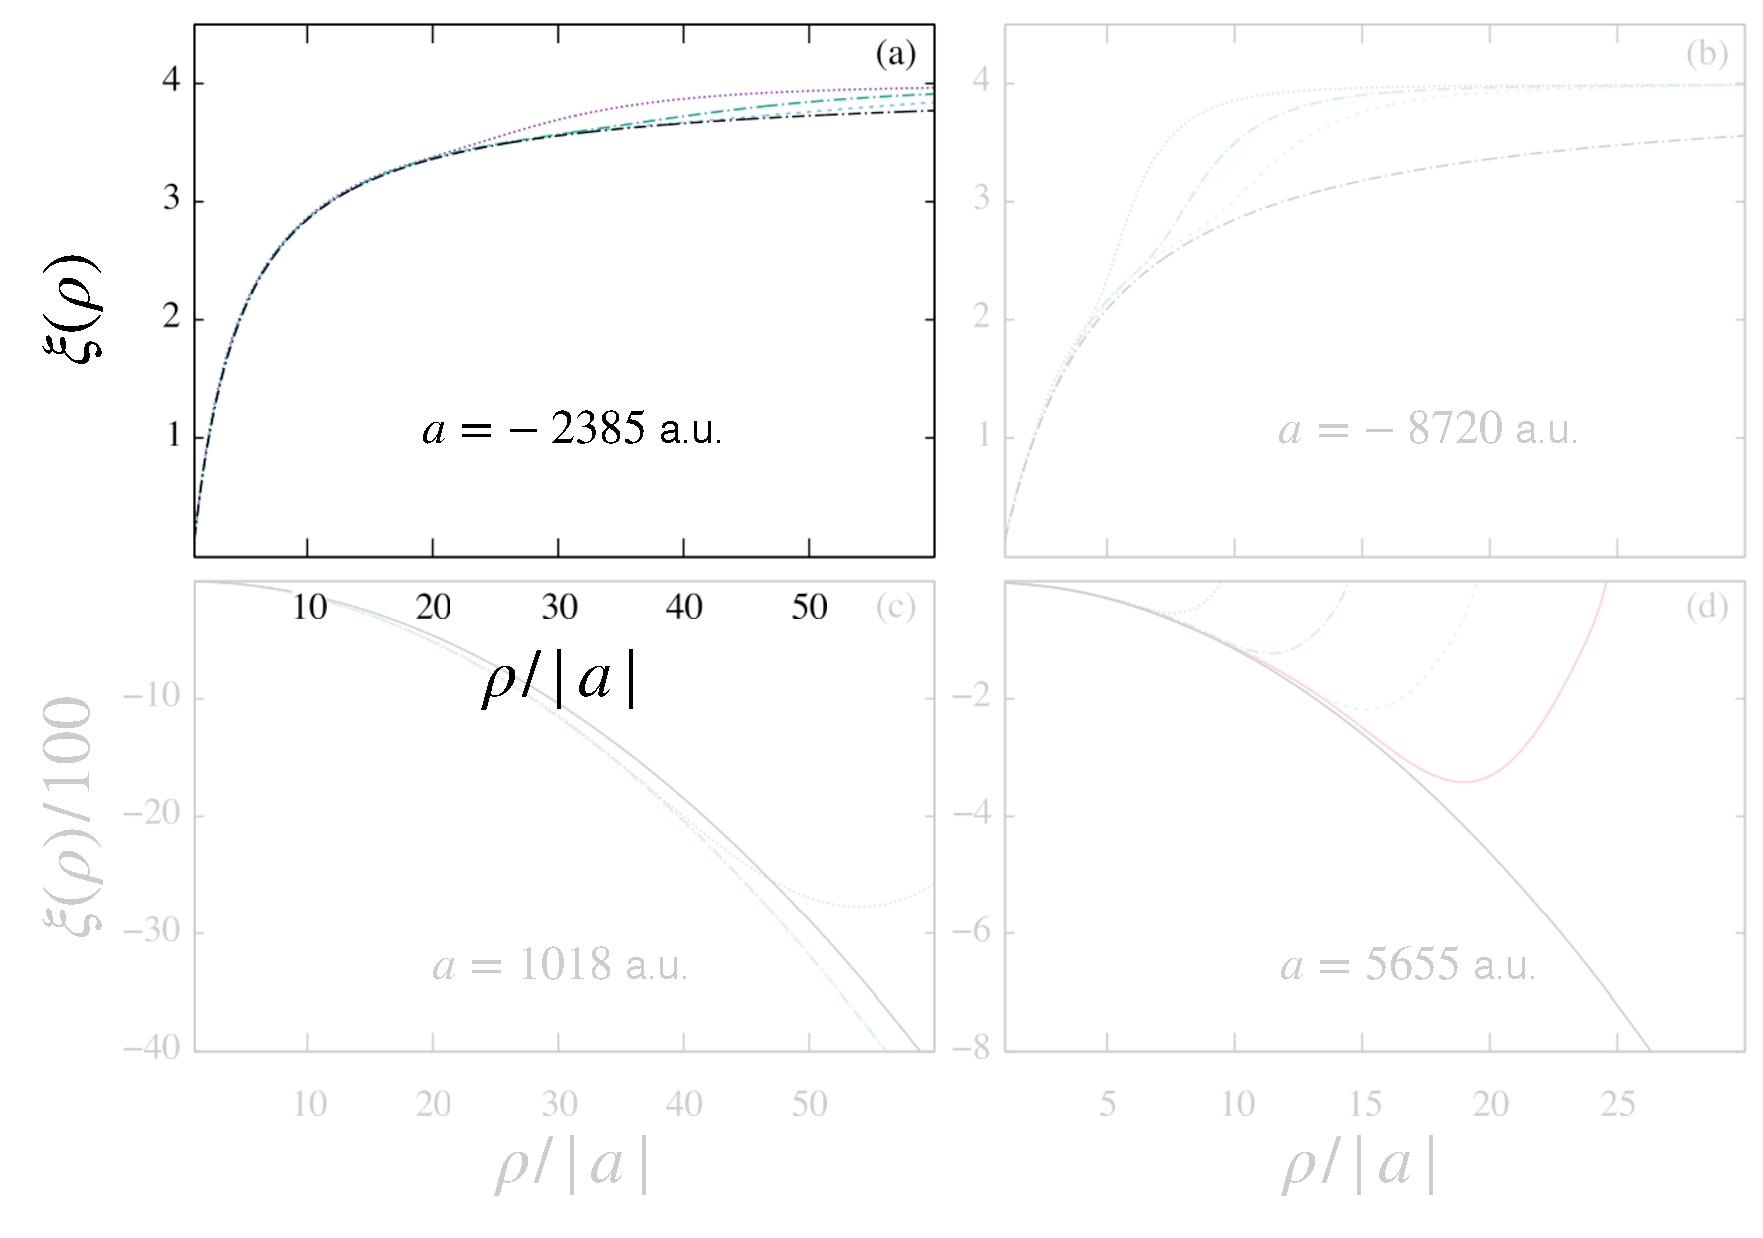
\includegraphics[width=1.0\linewidth]{neg1.pdf}}
	\only<2>{
	\hypertarget{neg2}
	\centering
	\vspace*{0.0cm}
	\hspace*{-0.2cm}
	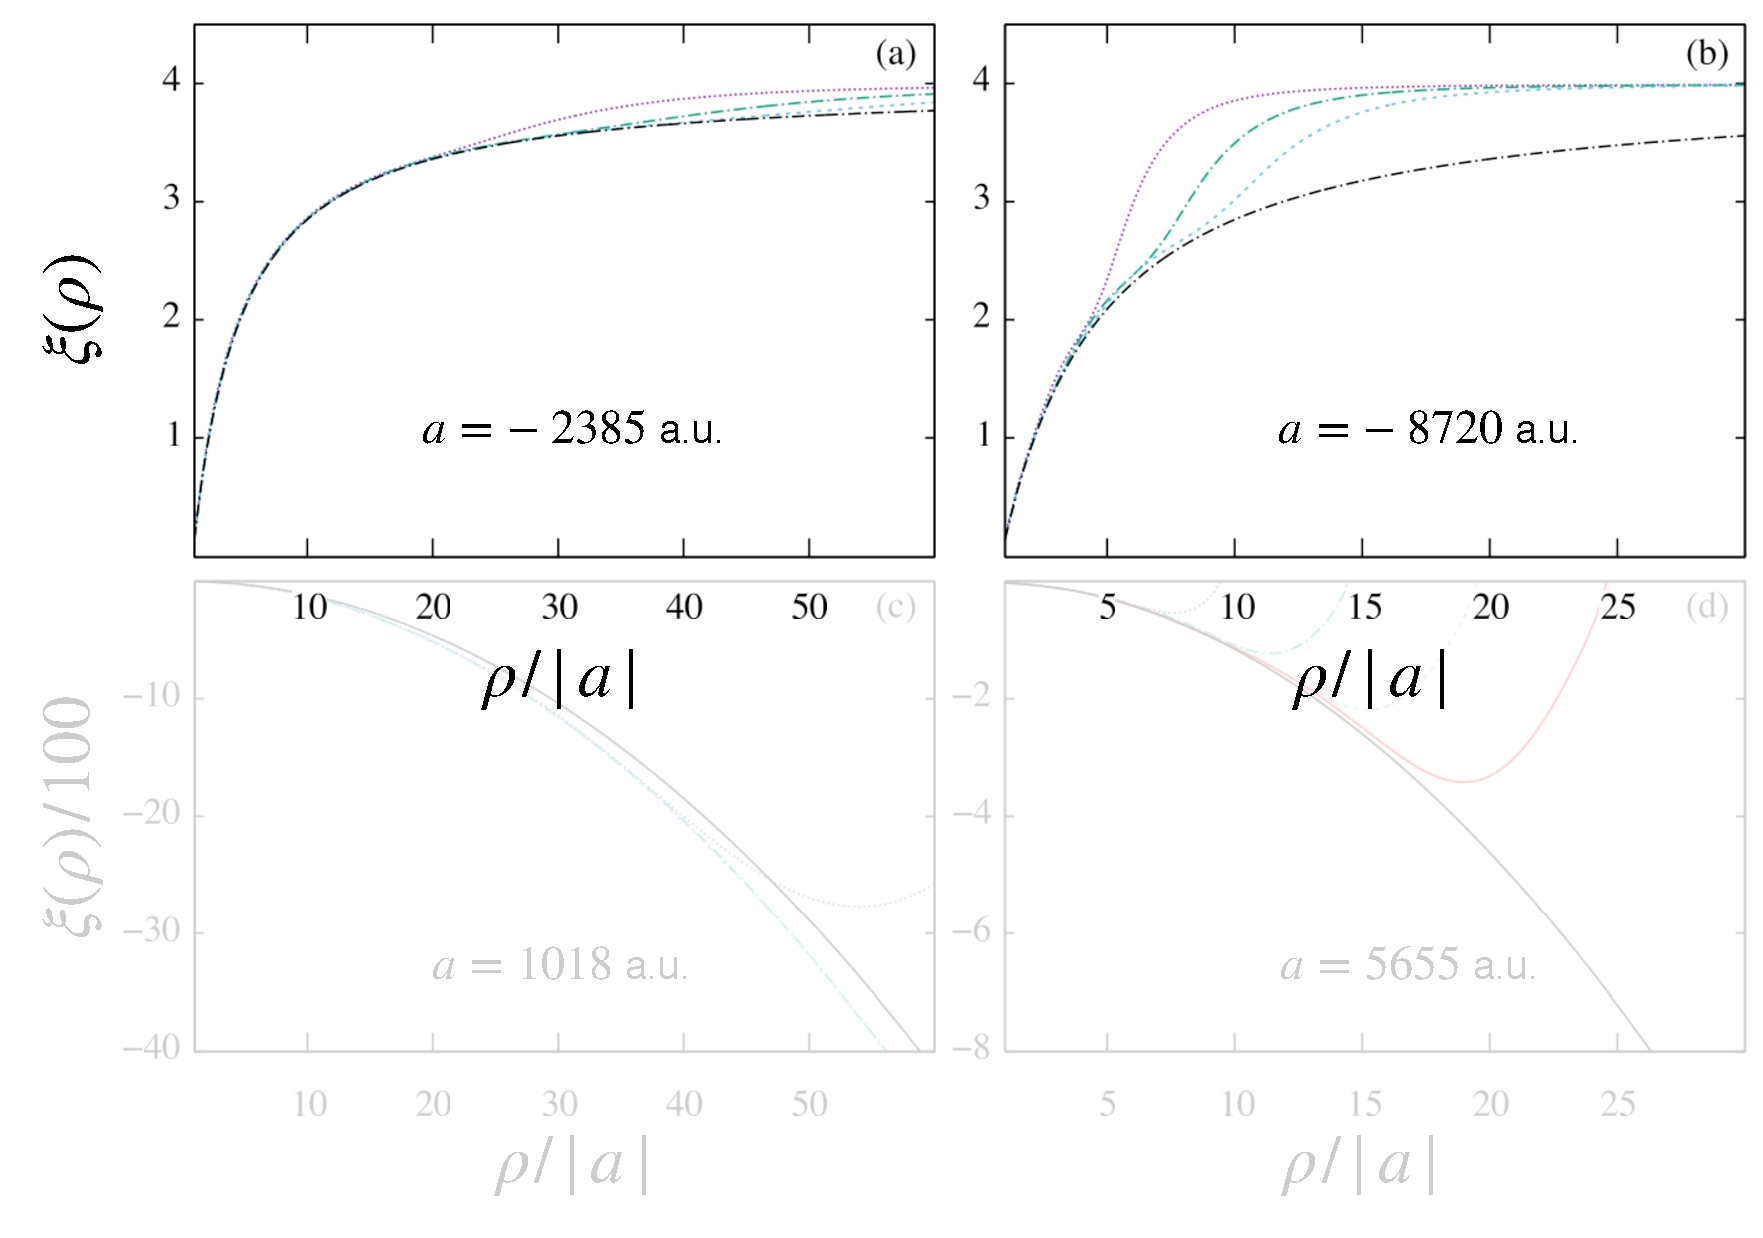
\includegraphics[width=1.0\linewidth]{neg2.pdf}}
	\only<3>{
	\hypertarget{pos1}
	\centering
	\vspace*{0.0cm}
	\hspace*{-0.2cm}
	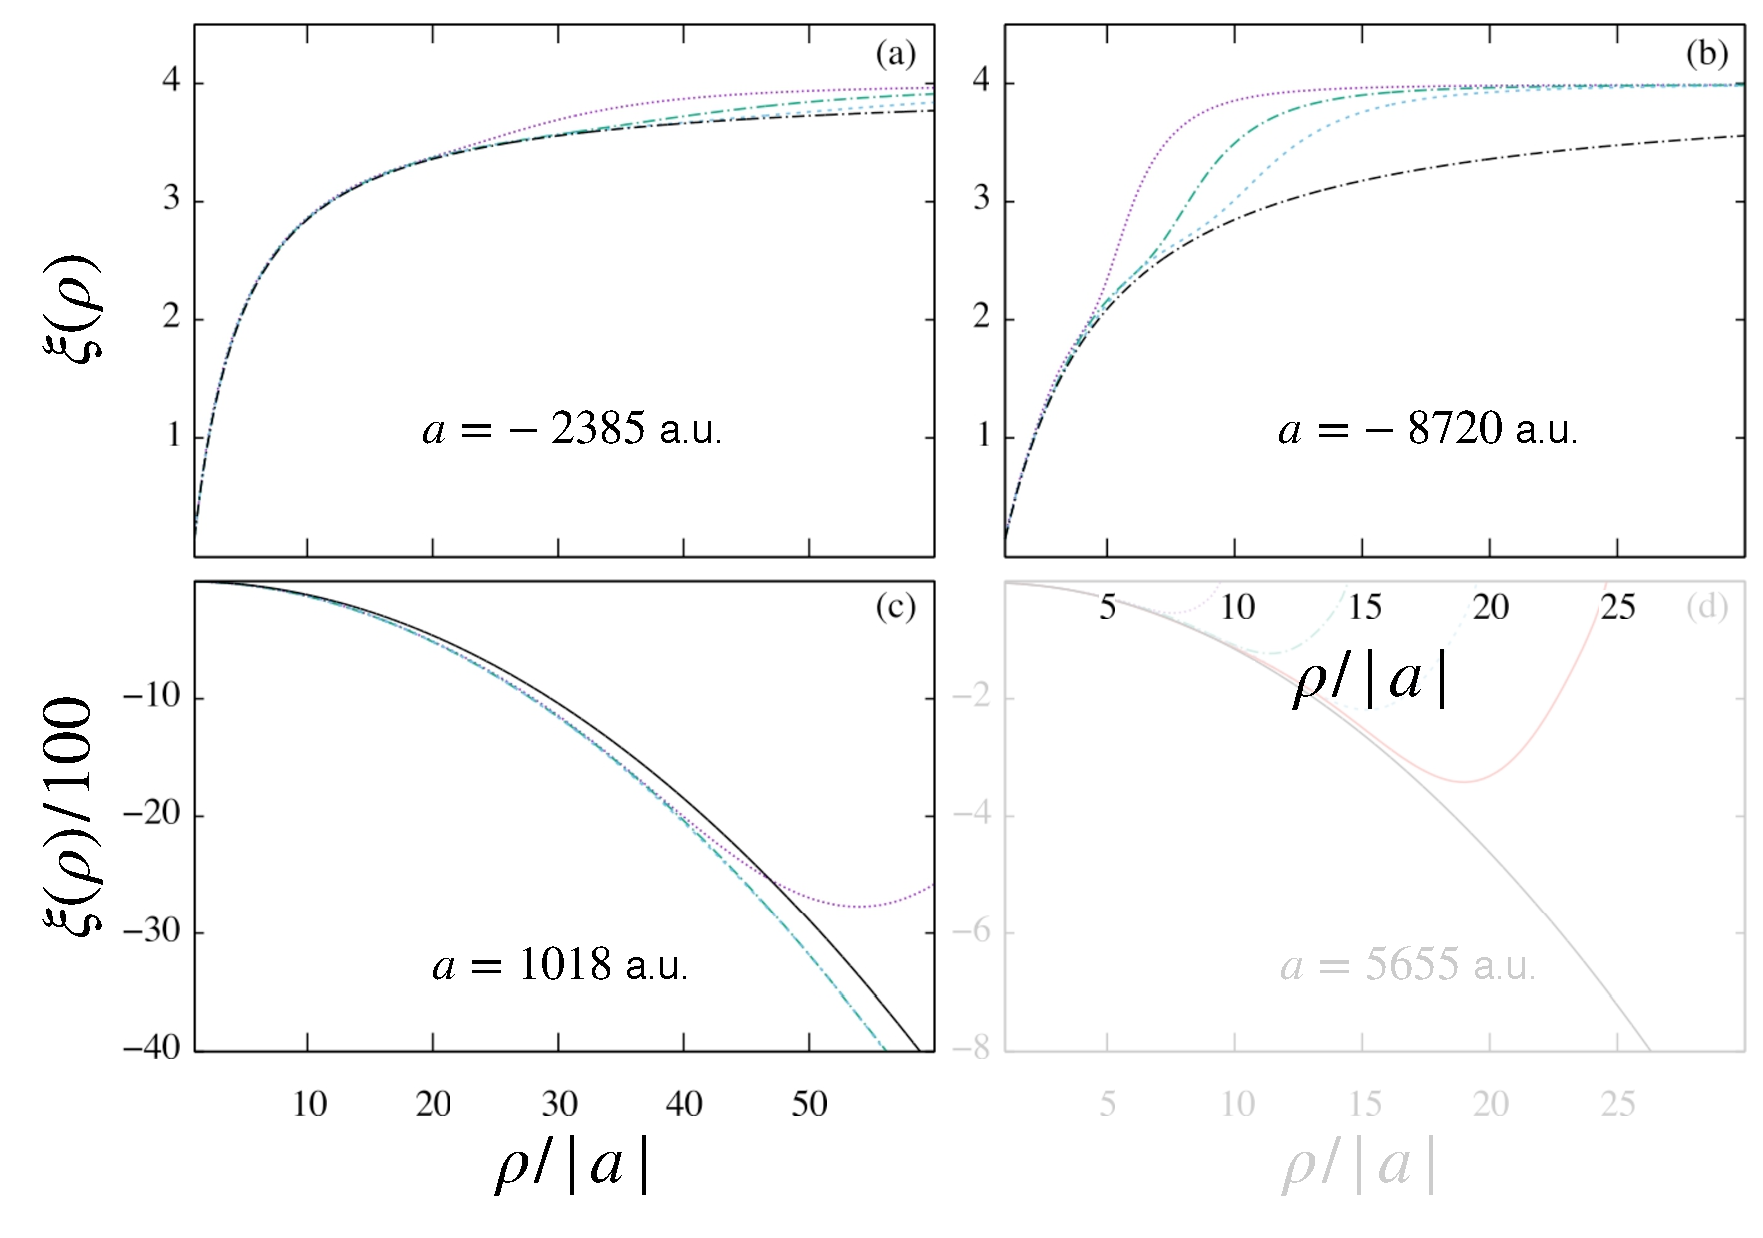
\includegraphics[width=1.0\linewidth]{pos1.pdf}}
	\only<4>{
	\centering
	\vspace*{0.0cm}
	\hspace*{-0.2cm}
	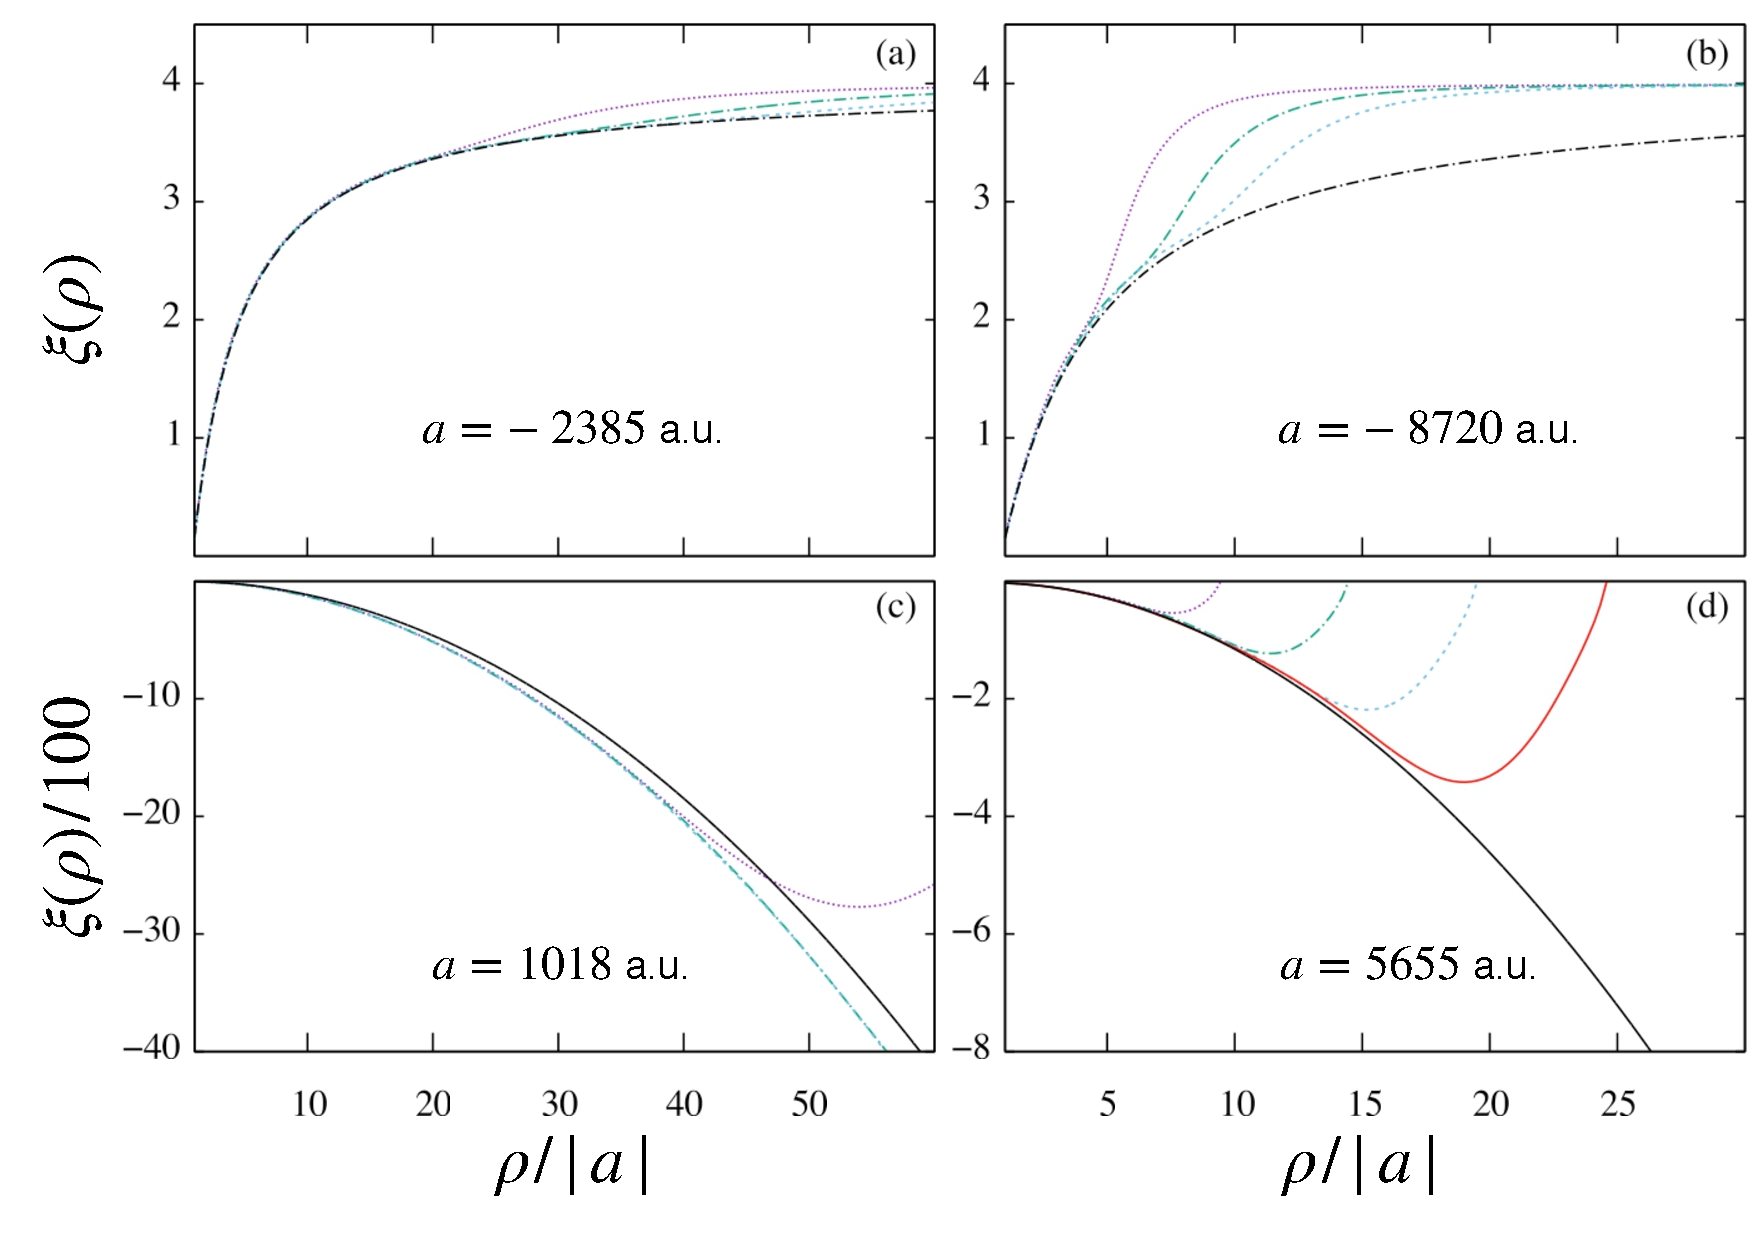
\includegraphics[width=1.0\linewidth]{pos2.pdf}}
	\only<5>{
	\hypertarget{lastres}
	\centering
	\vspace*{-0.1cm}
	\hspace*{-0.2cm}
	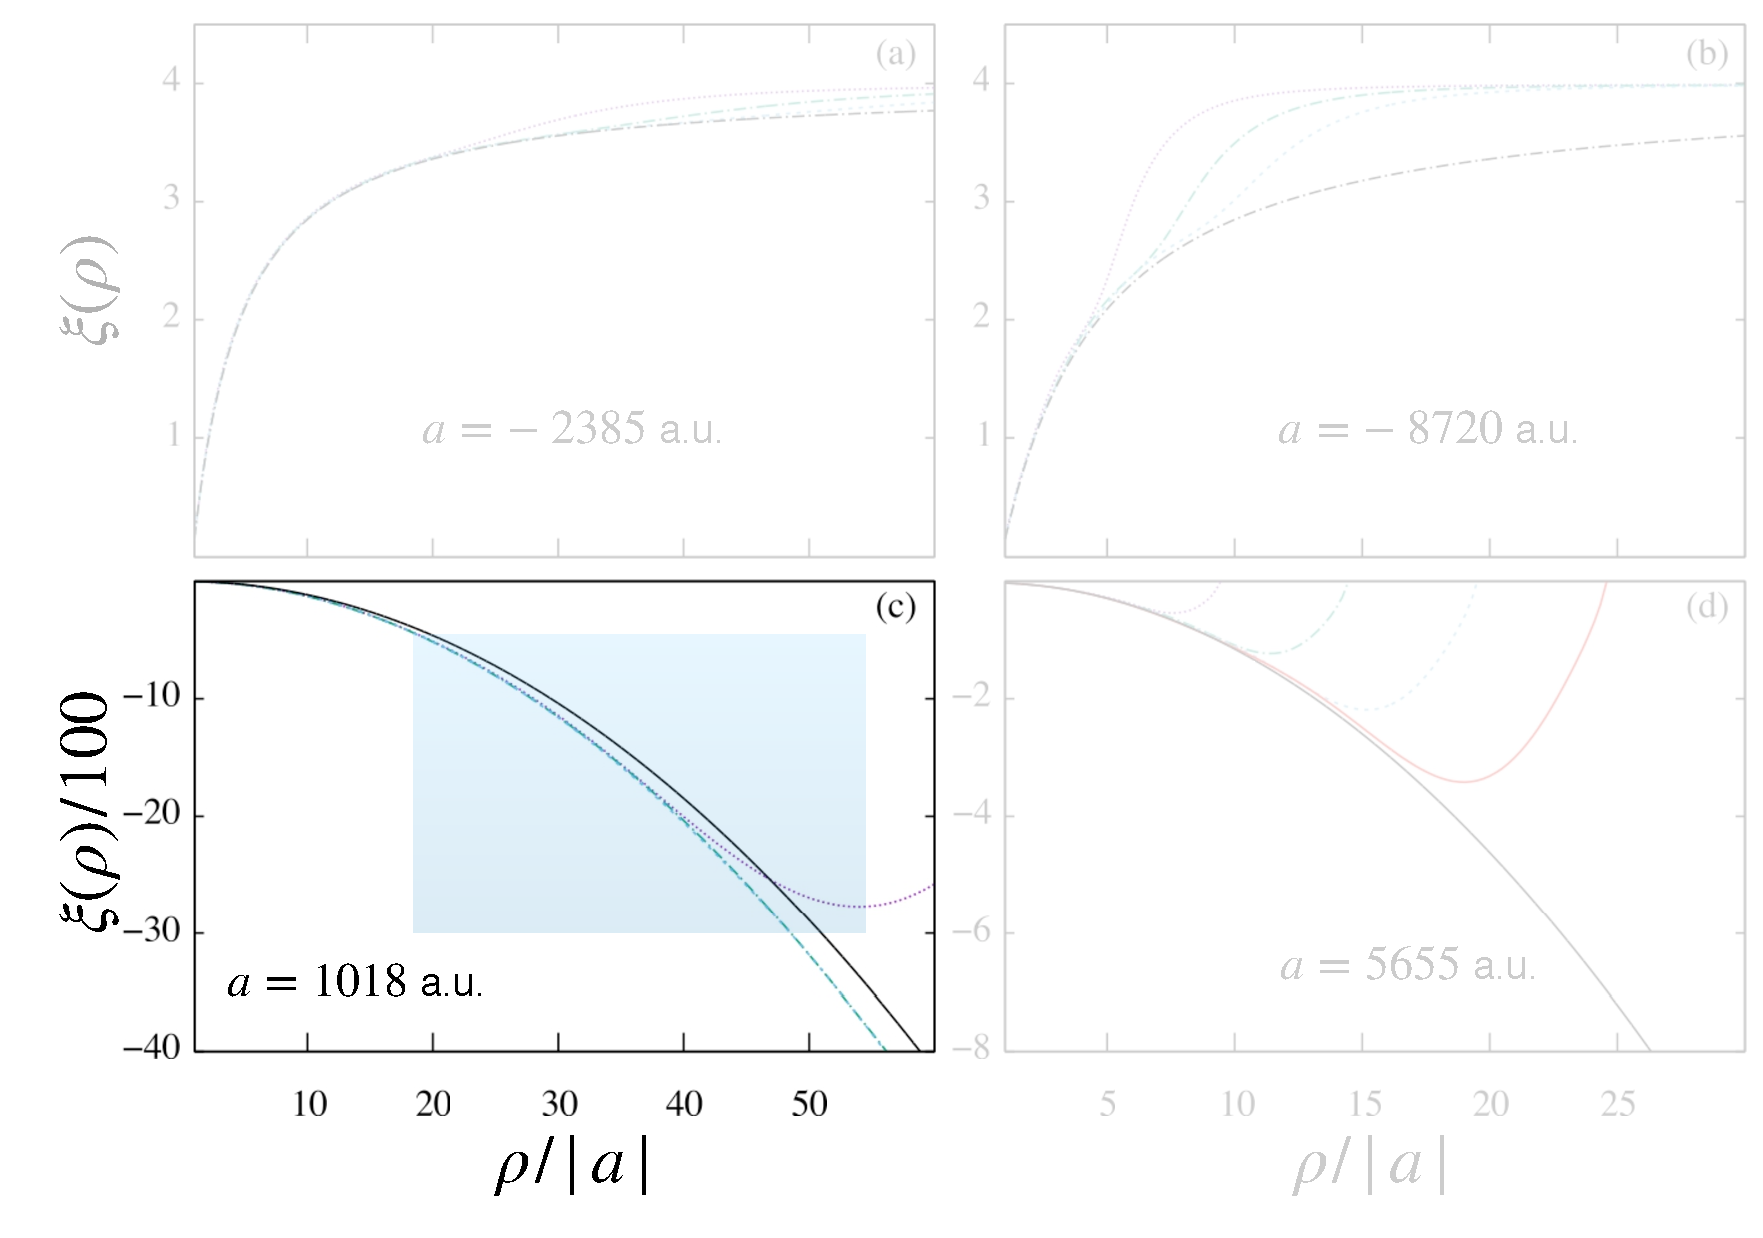
\includegraphics[width=1.0\linewidth]{pos3.pdf}}
	\begin{textblock*}{3cm}(12mm,1.15\textheight)%
	\hyperlink{R_faddeev}{\beamerreturnbutton{$\nu_0(\rho/a)$}}
	\hyperlink{dimer}{\beamerbutton{$E_{\mathrm{D}}$}}
   \end{textblock*}

\note[item]<1>{I have compared my numerically calculate potentials with the potential obtained solving the transcendental Faddeev eq.}
\note[item]<1>{I will show you the results for two negative and two positive $a$.}
\note[item]<1>{In this figure I have plotted the analytic potential (black dotted line) for negative $a$. The colored curves are numerical potentials calculated with an increasing number of B-splines in each direction. As might be expected the range of convergence is larger for potentials calculated with a largest number of B-splines.}
\note[item]<2>{We can observe that for larger magitudes of $a$ the range of convergence decreases.}
\note[item]<3>{No we look at positive $a$. Here we have the analytic curve in black. All numerically calculated potentials have converged over the whole hyppreradial range apart from the one calculated with the least number of B-splines.}
\note[item]<3>{However, there seem to be a small difference between the numerical and analytical results.}
\note[item]<4>{For larger $a$ the anlytical and numerical results show greater similarity.}
\note[item]<4>{However, again the hyperradial range of convergence have become smaller.}
\note[item]<4>{By comparing the panels to left and right, it appears that the hyperradial range for convergence generally is larger for the states with smaller $|a|$. We suspect that this discrepancy is due to the knot point placement, but this has not been verified yet.}
\note[item]<5>{Now, how do we this?}
\note[item]<5>{Well, the slightly different form in the parabolic divergency of the curves is due to a discrepancy between the exact two-body energy and the energy of the universal dimer.}
\end{frame}


%----------------------------------------------------------------------------------------

\begin{frame}
\frametitle{Comparison to the Analytical Model (3)}
\centering
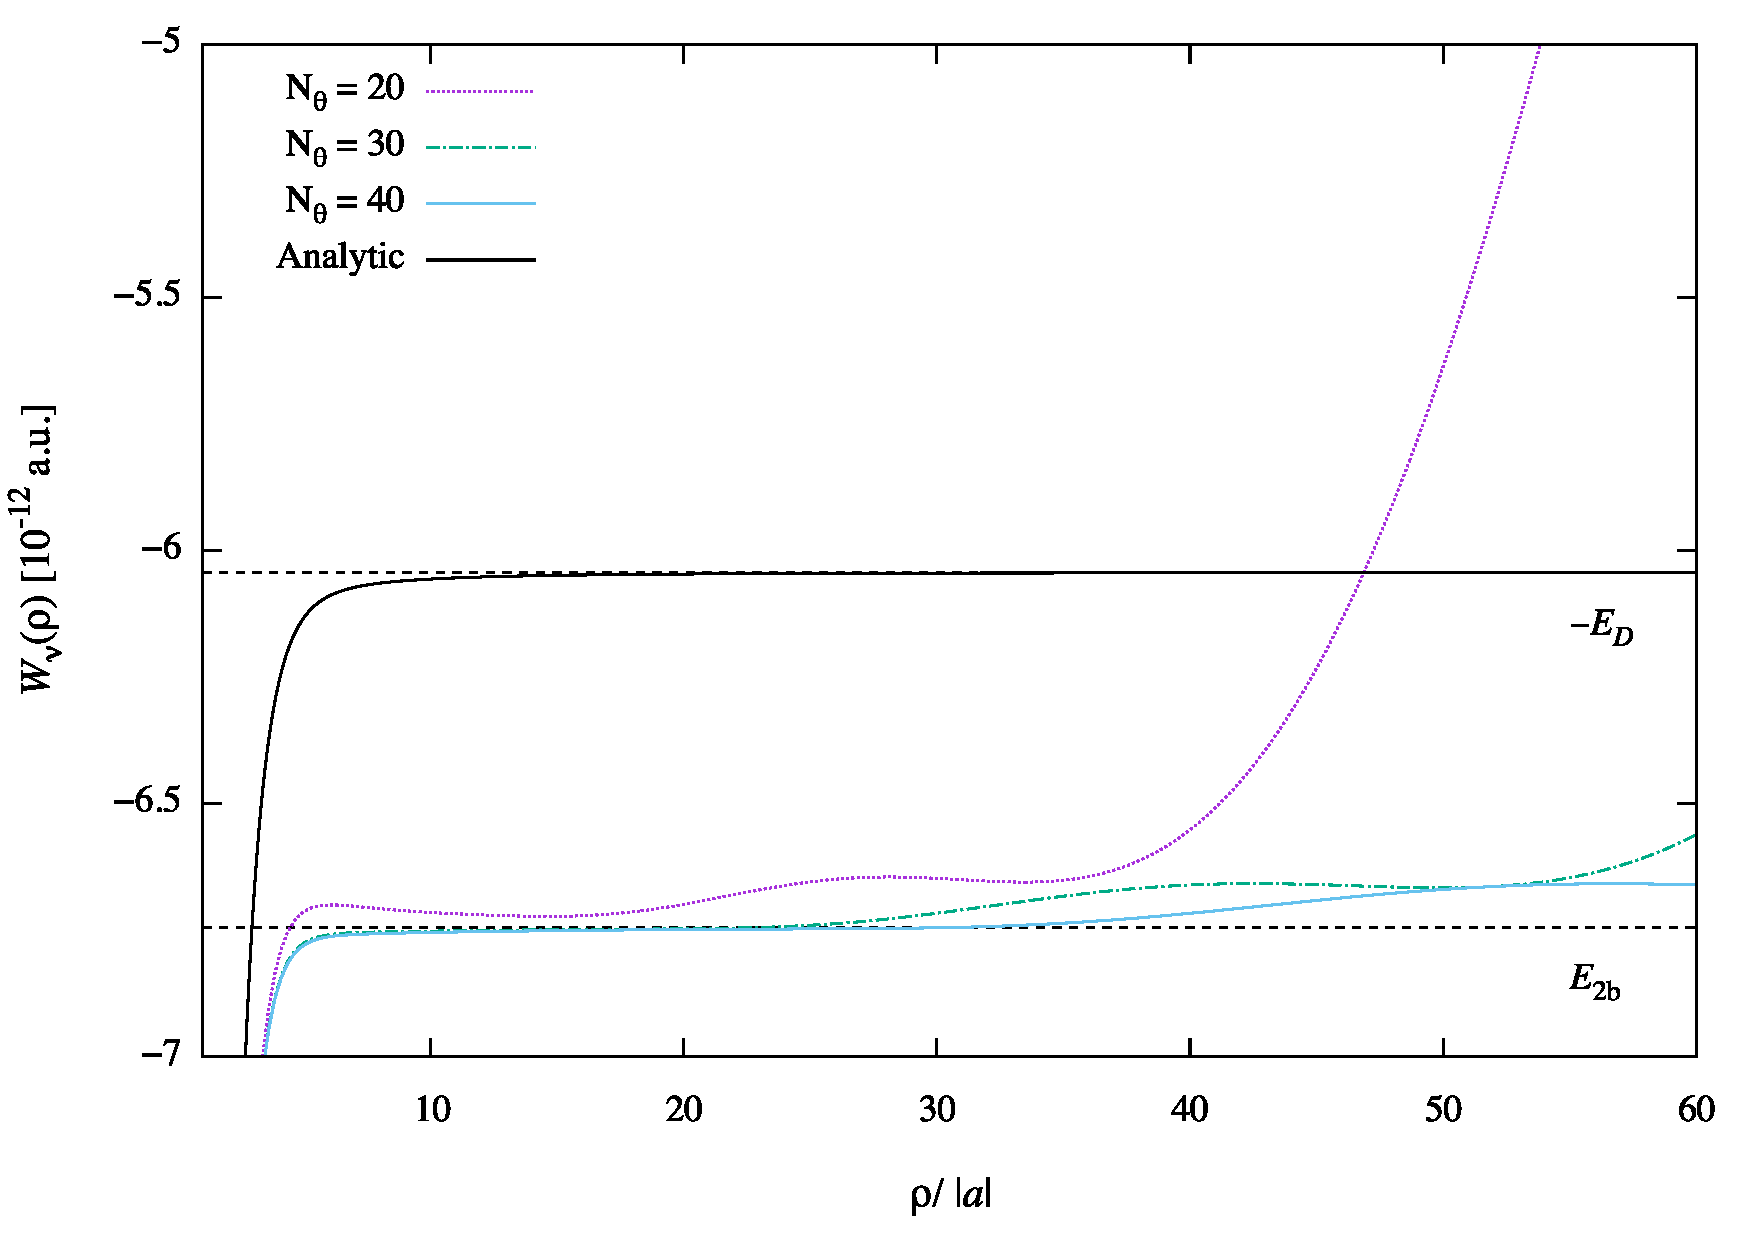
\includegraphics[width=1.0\linewidth]{twobodyenergy.pdf}
%\hyperlink{faddeev}{\beamerbutton{Faddeev}}
\note[item]<1->{Here I have plotted the actual three-body effective potentials $W$, the corresponding analytic potential together with the two-body energy $E_{2b}$ and the energy of the universal dimer.}
\note[item]<1>{We can see that the analytic potential goes to}
\end{frame}

\end{document} 